\documentclass[8pt, a6paper]{extbook}
\usepackage[left=12mm, right=10mm, twoside, top=10mm, bottom=8mm, includeheadfoot]{geometry}
\usepackage[cam, center, width=118mm, height=159mm]{crop}

\usepackage[sfdefault]{FiraSans}
\usepackage{FiraMono}
\usepackage{fontspec}
\usepackage{graphicx}
\usepackage{xcolor}
\usepackage{polyglossia}
\usepackage{needspace} % For avoiding orphan titles (country names)
\usepackage{xunicode}  % For \textcolor{}
\usepackage{xparse}    % For \NewDocumentCommand
\usepackage{hyperref}  % For \url{} and \href{}
\usepackage{titlesec}  % For \titleformat{}
\usepackage{pgffor}    % For \foreach{}
\usepackage[document]{ragged2e}  % For left-justified
\usepackage{fontawesome}
\usepackage{fancyhdr}  % For fancy headers
\usepackage[section]{placeins}

\setmainlanguage{esperanto}

\pagestyle{fancy}
\renewcommand{\sectionmark}[1]{\markboth{}{#1}}
\fancyhead[LO,RE]{\sectionmark}
\renewcommand\thesection{}     % Remove numbers
\renewcommand\thesubsection{}  % Remove numbers

\titleformat{\part}[hang]{}{}{0pt}{\centering\Geotica\large}
\assignpagestyle{\part}{empty}
\setmainfont{Fira Sans}

\newfontfamily\semibold{Fira Sans Medium}
\newfontfamily\light{Fira Sans Light}
\newfontfamily\lightitalic{Fira Sans Light Italic}
\newfontfamily\Geotica[Scale=3]{Geotica Three}
\setlength\parindent{0pt}  % No paragraph indentation
\definecolor{light-gray}{gray}{0.8}
\hypersetup{colorlinks=true, citecolor=black, filecolor=black, linkcolor=black, urlcolor=black}

\newcommand*\blankpage{\newpage\thispagestyle{empty}\null\newpage}
\newcommand*{\name}[2]{#1 \textsc{#2}}
\newcommand*{\eastname}[2]{\textsc{#2} #1}
\NewDocumentCommand\invisiblesection{ s m }{%  {star, mandatory}
  \refstepcounter{section}%
  \sectionmark{#2}%
    \IfBooleanF#1{%  % If no star is seen
      \addcontentsline{toc}{section}{\protect\numberline{\thesection}#2}}}

\begin{document}
  
    
{
  \titleformat{\section}[block]{}{}{0pt}{\centering\huge\textbf}
  \titlespacing{\section}{0pt}{4em}{1em}
  \titleformat{\subsection}[block]{}{}{0pt}{\large\textbf}
  \titlespacing{\subsection}{0pt}{2em}{1em}
  \titleformat{\subsubsection}[block]{}{}{0pt}{\small\textbf}
  \titlespacing{\subsubsection}{0pt}{0pt}{0pt}
  \hyphenpenalty=10000\relax  % No hyphenation

  
    \thispagestyle{empty}
    \part*{Adresoj}
  

  

  
    {{ country.grouper.name|cmd:"section" }}
      \vspace{.6em}\nopagebreak
      
        
            {\small
            {\semibold
                Landa OrganizantoLandaj Organizantoj
            }\nopagebreak
            
                {{ profile|full_name }}
                {{ profile.email|escape_latex|cmd:"texttt"|ctx:"footnotesize" }}
            
            }
        \vspace{.7em}
        
      

      
      
        {{ region.grouper|safe|cmd:"subsection*" }}{# TODO: display region's Esperanto or latin name #}
        
          {{ city.grouper|safe|cmd:"subsubsection" }}
            
              \begin{minipage}{\textwidth} {# Address block won't break with minipage #}
              {\small
                {{ place.owner.get_title_display|ctx:"light" }}{# TODO: display also the gender; show only non-deleted (and non-hidden) family members. #}
                {{ place.owner|full_name }}~{{ place.owner.birth_date.year|bracket|ctx:"light" }}, {{ member.first_name }}~{{ member.birth_date.year|bracket|ctx:"light" }}:
                  {{ place.get_postcode_display|escape_latex }}~{{ place.city|escape_latex|ctx:"semibold" }}
                  {{ place.address|escape_latex }} {# TODO: show non-deleted phone numbers according to visibility settings and sorted by importance. #}
                  {{ phone.latex }} {{ phone.comments|escape_latex|ctx:"lightitalic,footnotesize" }} 
                {{ place.owner.email|escape_latex|cmd:"texttt"|ctx:"footnotesize" }}
                  {{ place.max_guest }}g\,\,{{ place.max_night }}n\,\,{{ place.contact_before }}t
                  {{ place.short_description|escape_latex|cmd:"light" }}
                {{ place.conditions.all|join:" " }}
              }
              \vspace{.5em}
              \end{minipage}
            
          
      
      
        
      
  

}

  
    \frontmatter\pagenumbering{Roman}
    
\begin{titlepage}
  \begin{center}
    \vspace*{10mm}
    {\Geotica
      {\huge Pasporta\\ Servo}

      \vspace{20mm}

      {\huge \textasciitilde}

        \vspace{24mm}
        {{ year|ctx:"small" }}
    }
  \end{center}
\end{titlepage}

    \invisiblesection{Kolofono}
{\parskip=.6em

Pasporta Servo 2017\\
ISSN: \texttt{1879-7598}\\
\today

{\normalsize
\begin{description}
  \item[\name{Baptiste}{Darthenay}] Kompilanto, Ĉefprogramisto
  \item[\name{Stela}{Besenyei-Merger}] Ĉefadministranto, Kunordiganto\\ de Landaj Organizantoj
\end{description}

\subsubsection{Dankoj}
    \name{Meiyer}{Goren} \hfill
    \name{Roy}{McCoy} \hfill
    \name{Alexandre}{Baudry} \hfill
    \eastname{Veronika}{Poór}

\quad

\textbf{Tutmonda Esperantista Junulara Organizo}\\
Nieuwe Binnenweg 176 \hfill +31 10 436 1044\\
NL-3015 BJ Rotterdam \hfill \texttt{oficejo@tejo.org}

Estrarano pri Pasporta Servo: \name{Juliana}{Evandro}

Komisiito de Pasporta Servo:\\
  \quad 2016 — \name{Lars}{Sözüer}\\
  \quad 2017 — \name{Stela}{Besenyei-Merger}

Ilustraĵoj: \name{Robin}{Guinin}, Francio

Provlegado: \name{Anna}{Besenyei}

Prespretigo: \name{Baptiste}{Darthenay}

Presado: Skonpres, Pollando

\newfontfamily\cmr[Scale=1.3]{cmr10}
Kompostita per Liberaj Programaroj sur GNU/Linukso:\\
{\cmr \LaTeX}, Python, Django, PostgreSQL, Inkscape, Scribus, QGIS

}


\newpage
\vspace*{3em}
\thispagestyle{empty}
{\Large\light ~\hfill Tiu libro apartenas al:}\\
\vspace{4em}
\textcolor{light-gray}{\hrulefill}

    \thispagestyle{empty}
\begin{figure}[p]
    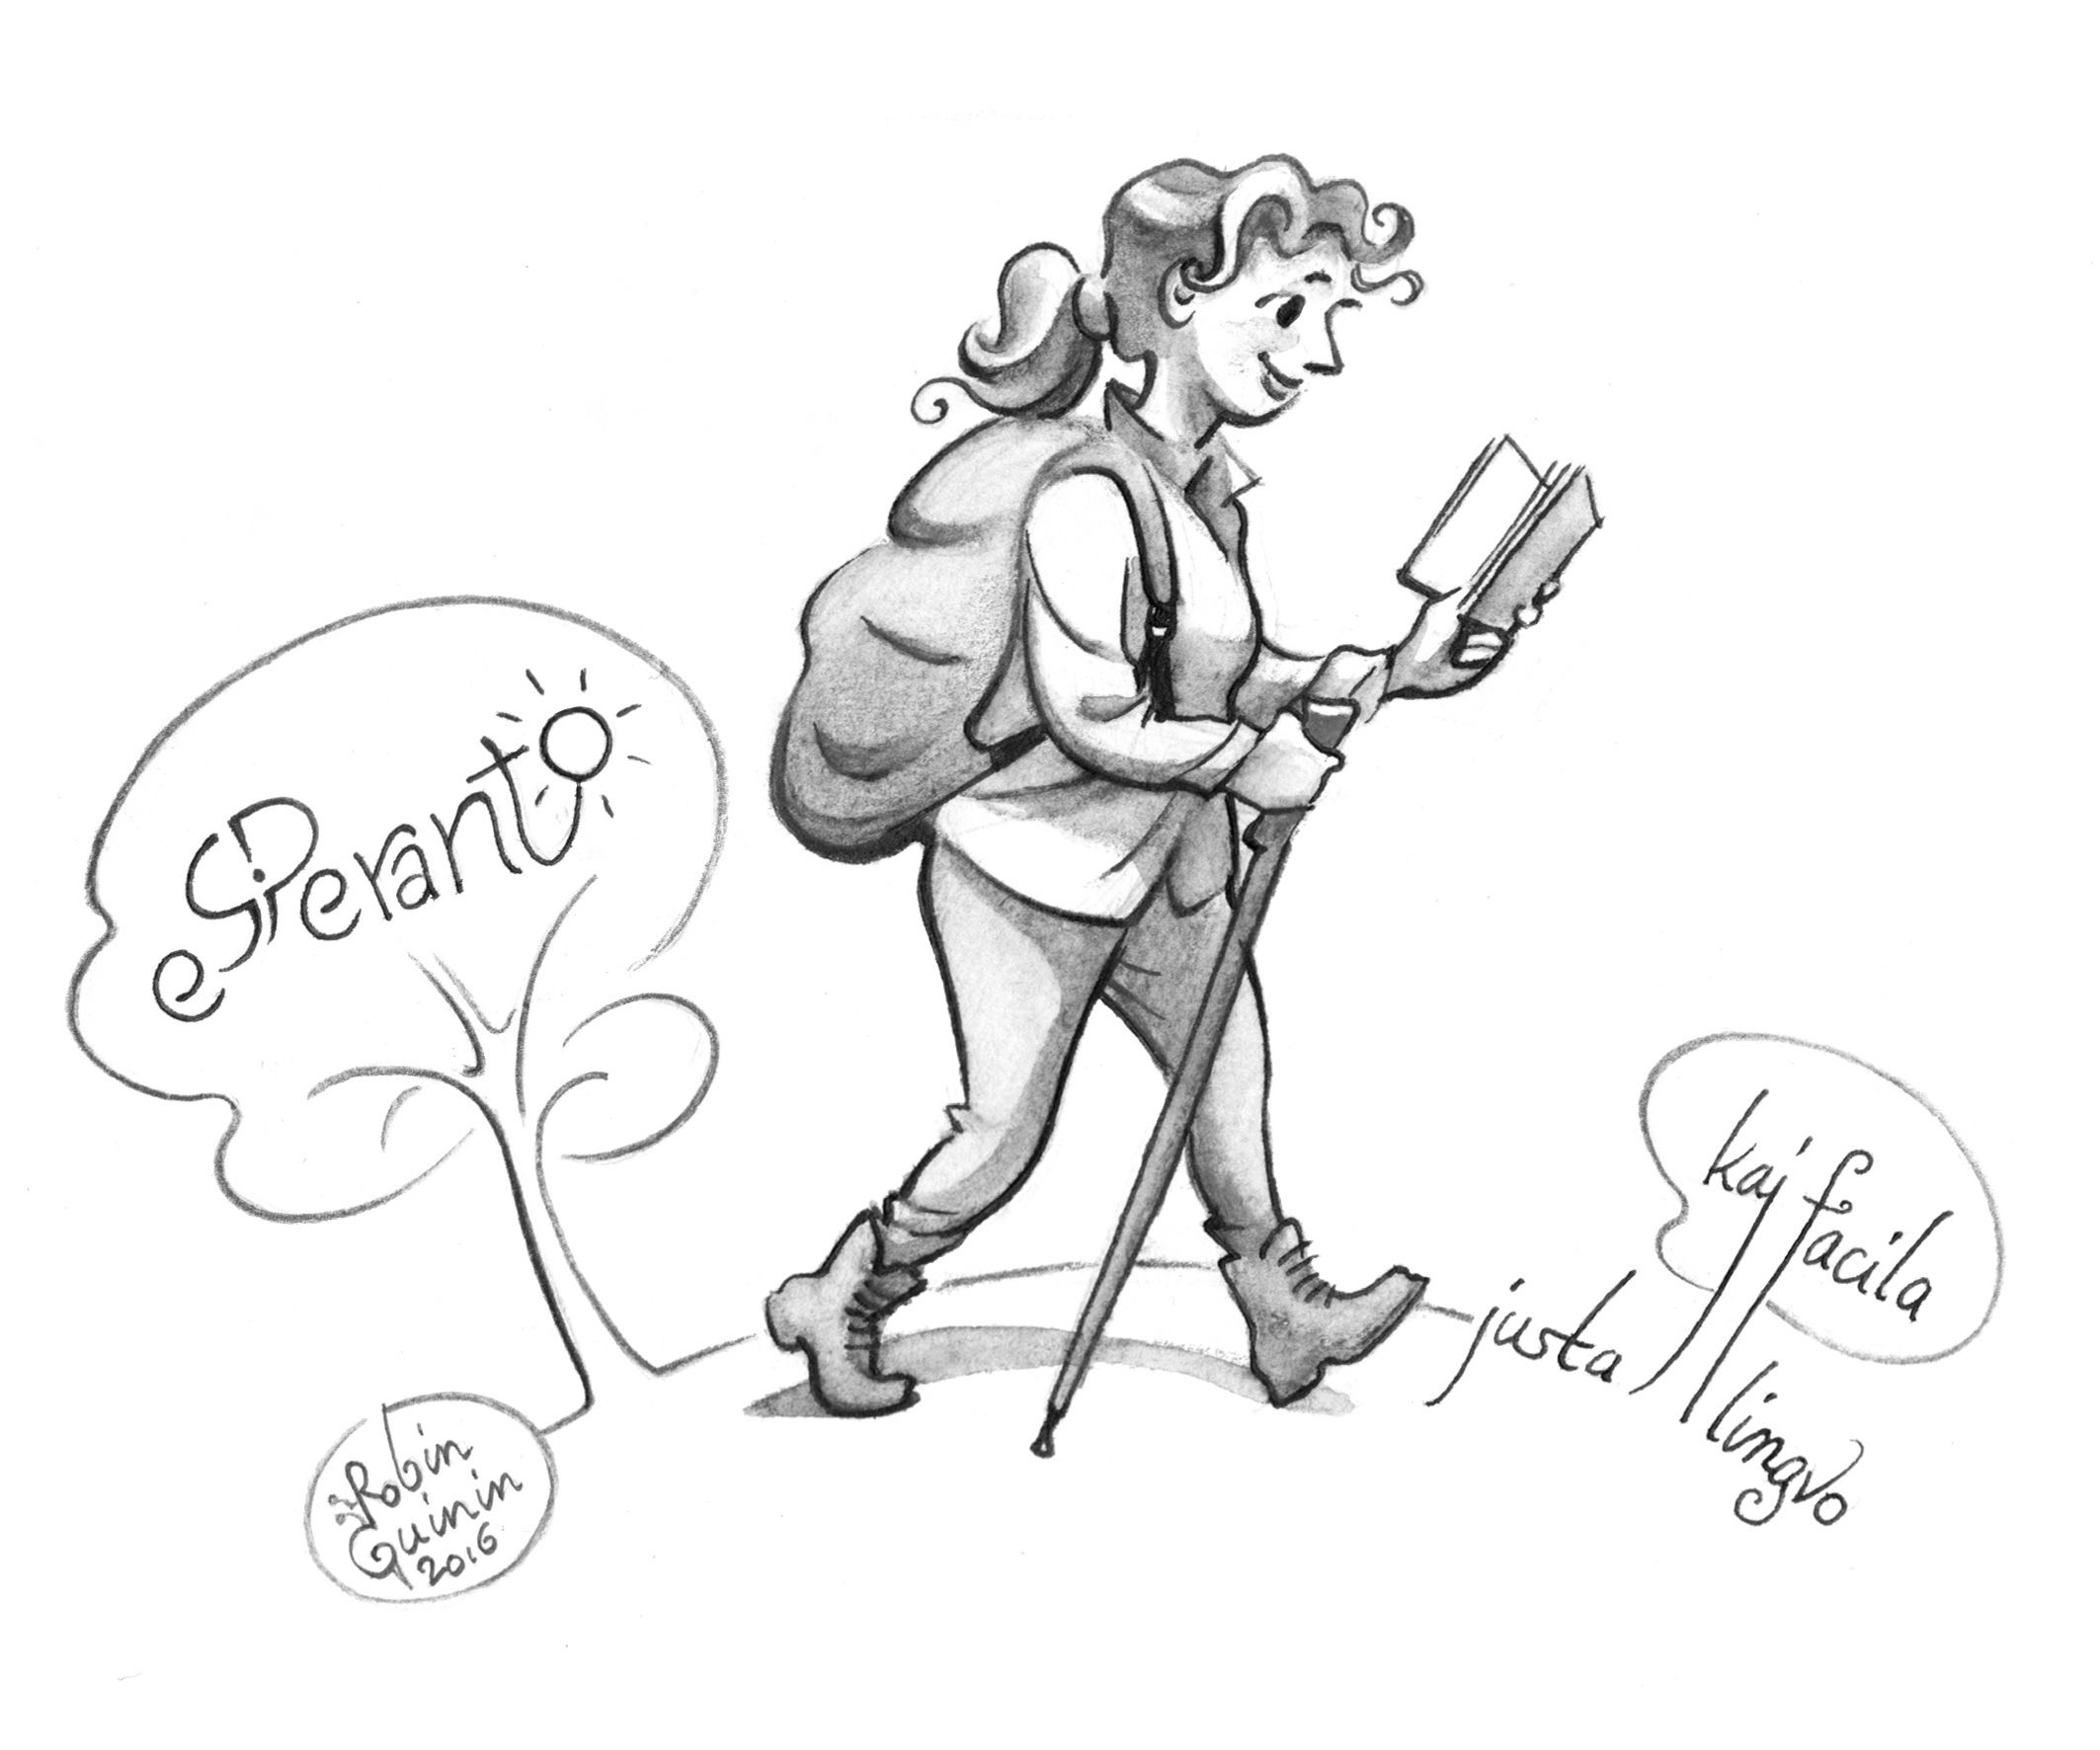
\includegraphics[width=\textwidth]{img/PS_2017_1_enkonduko.jpg}
\end{figure}

    \invisiblesection{Prefaco}
\thispagestyle{plain}
{\parskip=1em

Karaj gastoj kaj gastigantoj!

\vspace{.8em}

En la Jaro de Zamenhof, 2017 Pasporta Servo reviviĝas kaj revenas en niajn vivojn. Vi denove povas teni la libron en viaj manoj!

Pasporta Servo praktike signifas, ke tiuj homoj kiuj gastigas akceptas homojn en sia hejmo por almenaŭ unu nokto senpage. Sed la komunumo de Pasporta Servo estas multe pli ol nur la sumo de tiuj pasigitaj noktoj tutmonde. Estas multege da Esperanto-parolantoj, kiuj lernis la lingvon pro Pasporta Servo. Ili unue uzis ĝin por vojaĝi, kaj nun jam mem kiel gastigantoj enestas. Vi trovos gastigantojn, kiuj jam enestis 30 jarojn antaŭe ankaŭ kaj daŭre entuziasme gastigas.

Ni scias, ke ne ekzistas Esperanto-lando, do ni mem devas krei la oportunojn por renkontiĝi, uzi nian lingvon. Vojaĝado, ekkonado de landoj tra la okuloj de lokanoj, esti akceptata en la hejmo kiel malnova amiko estas multe pli ol simple listo de adresoj sugestas.

Pasporta Servo, la libreto revenas post iom longa silento. Tamen, intertempe multe da aktivuloj strebis restarigi la sistemon. Uzis sociajn retejojn aŭ aliajn gastigoservojn por gardi la spiriton de gastigado de Pasporta Servo. Dankon al vi!

La libreto revenas, kaj estas multege da laboro malantaŭ ni. Multaj demandas min: kial gravas la libro nun, en 2017? Kiel ne sufiĉas la retejo aŭ apo por poŝtelefono? La respondo estas facila: ĉi tiu libro enhavas nur plene konfirmitajn adresojn, nur homojn kiuj daŭre deziras resti gastigantoj. Kiuj estas en la libro, ĉiu persone respondis al niaj leteroj aŭ alvokoj.

En la retejo estas multe pli da gastigantoj, kaj ni provis kontroli kiom eble plej multe, sed tiuj, kiuj aperas ĉi tie rapide respondas, emas gastigi, kaj elkore bonvenigas vin. Vi volas tiajn gastigantojn, ĉu ne?

Tamen ankaŭ la retejo bone funkcias. Jam plurmil personaj mesaĝoj estis senditaj ekde la relanĉo en novembro 2014. Do, nun venas la tempo danki la kompilanton de la libro, kaj ĉefprogramiston de la projekto: \name{Baptiste}{Darthenay}, kiu persone faris pli ol tri kvaronojn de la tuta projekto, kaj pro kiu vi nun povas teni la libron en viaj manoj.

Mi tre dankas la laboron de la Landaj Organizantoj kaj helpantoj, kiuj kontaktis la gastigantojn. Dankon al TEJO, ke kunlabore kun UEA dungis Baptiste kaj min por 4 monatoj, tiel ni povis trankvile labori interalie pri la libreto.

Fine, dankon al la gastigantoj kaj vi, ke vi aĉetis la libron! Sciu, ke tiel vi rekte subtenas Pasportan Servon.

Ni daŭre laboros por evolui la libron, la retejon kaj la komunumon de Pasporta Servo. Ni esperas, ke la libro eĉ pli vigligos la Esperanto-komunumon kaj kontribuos al neforgeseblaj vojaĝoj, renkontiĝoj, kaj babiladoj!

Bonvenon al Pasporta Servo 2017!

\vspace{.8em}

~\hfill\textit{\semibold Stela}
}

    {\pagestyle{plain}
    \invisiblesection*{Enhavo}
    \tableofcontents
}

    \mainmatter
    \thispagestyle{plain}
{
  \titleformat{\section}[block]{}{}{0pt}{\huge\textbf}
  \parskip=0.6em

\section{Enkonduko}

\subsection{Kio estas Pasporta Servo?}


Pasporta Servo estas plene volontula internacia gastiga servo per Esperanto. Ĝi estas la ilo, kiu enhavas la gastigantojn, kiuj pretas oferti senpagan tranokteblon en siaj hejmoj por almenaŭ unu nokto. Praktike ĝi estas listo de adresoj ordigitaj laŭ landoj laŭ la Esperanta alfabeto.

Pasporta Servo permesas multe malpli koste vojaĝi tra la mondo. Kie kaj laŭ kiuj kondiĉoj vi tranoktas dependas de la gastiganto. Kelkfoje vi havos nur lokon sur planko, aŭ matracon, sed povas okazi, ke eĉ liton aŭ apartan ĉambron!

Vi aldone povas ricevi helpon de la lokanoj rilate al la restado en la lando: pri transporto, kiujn lokojn viziti, kion manĝi, provi, sperti.

\subsection{La komencoj de Pasporta Servo}

La unua ideo pri la tiel nomata \textit{Programo Pasporto} estiĝis en 1966, de \name{Ruben}{Feldman-Gonzalez} el Argentino. Pasporta Servo laŭ la nuna sistemo aperis unuafoje en 1974, kun 39 gastigantoj, sub gvido de \name{Jeanne-Marie}{Cash} el Francio. Ambaŭ pioniroj daŭre estas gastigantoj de Pasporta Servo.

Pasporta Servo estas eldonaĵo de la Tutmonda Esperantista Junulara Organizo (TEJO).

\subsection{Kial estas utila Pasporta Servo por la gastiganto?}

Por gasto havi tranokteblon senpage estas bonege. Havi gastiganton kun kiu oni povas facile interkompreniĝi parolante Esperanton eĉ pli bone. Tamen Pasporta Servo helpas ankaŭ la gastigantojn. Kelkaj gastigantoj ofte ne havas mem la eblon vojaĝi, praktiki la lingvon aŭ partopreni Esperanto-renkontiĝojn. Do, Pasporta Servo donas la eblecon interligi Esperanto-parolantojn. Tiel vi povas lerni pri aliaj kulturoj ne nepre devante vojaĝi. Konsideru iĝi gastiganto!

\subsection{Kiel vi povas membriĝi en Pasporta Servo?}

Unue, se vi estas gastiganto, vi aŭtomate estas membro de Pasporta Servo.
Se vi deziras gasti, vi jam tenas tiun libron en via mano. Certiĝu, ke vi skribas vian nomon sur la kovrilon!
Nia retejo: www.pasportaservo.org/registrado/ estas tre facile uzebla, vi povas kaj registri vian hejmon, kaj serĉi gastigantojn. Vi iĝas membro plenigante viajn datumojn.
Membreco en Pasporta Servo ne estas ligita al iu ajn alia membreco.
La servo mem estas senpaga, sed ne senkosta. Aĉetado de la libro subtenas la projekton, kaj ajna monsumo helpas pagi la laboron de la programistoj, redaktoroj, presadon de la libro kaj la servilon.

Tra UEA vi povas mendi pliajn PS-librojn aŭ subteni nian laboron per ajna monsumo.
Por vidi pri la pagado, bv. iru al:\\
http://www.uea.org/alighoj/pagmanieroj

Dankon pro via subteno!


\subsection{Kiel vi povas fariĝi gastiganto?}

Vi fariĝas gastiganto aŭ membriĝante ĉe pasportaservo.org aŭ sendante viajn informojn al Centra Oficejo de TEJO. Via aliĝilo devas alveni ĉe la kompilanto antaŭ la limdato indikita sur la aliĝilo por esti certa pri apero en la sekva eldono de Pasporta Servo.

Se vi havas ajnan problemon rilate al la registriĝo, nepre skribu al saluton@pasportaservo.org, ni volonte helpas al vi!

\subsection{Bazaj kondiĉoj}

La plej grava kondiĉo estas, ke ĉiu membro de Pasporta Servo (gastoj kaj gastigantoj) devas paroli Esperanton. Tio estas la bazo de la Servo, kaj ĝi estas nenegocebla. Povas okazi, ke vi ne parolas tre bone, sed vi devas povi komuniki en Esperanto.

Tiu kondiĉo ne estas nepra por kunloĝantoj kaj kunvojaĝantoj, krom se gastiganto mencias en siaj kondiĉoj, ke akceptas nur Esperanto-parolantajn gastojn.

La gastiganto devas oferti minimume unu nokton senpage por ĉiu gasto. Povas eventuale peti monon kontraŭ matenmanĝo aŭ aliaj servoj, sed tio devas esti klare skribite en la kondiĉoj aŭ strikte nur laŭ interkonsento antaŭ la alveno.

Ĉiu kondiĉo de la gastiganto devas esti respektita. Memoru, temas pri fido kaj bonvolo. Se vi ion ne komprenas, aŭ pri io ne certas, prefere demandu la gastiganton por klarigo.

La gasto neniam rajtas alveni sen antaŭa kontaktado. Se tio okazas, ne surprizu, se vi, la gasto estos forsendita.


\subsection{Ĝis kiam validas la libro?}

Ĉiu adreslibro validas ĝis la sekva eldono. Ĝi devas aperi ĉiu jare, la adresoj validas en la jaro, kiu troviĝas sur la kovrilo.

\subsection{Konfirmado de la adresoj}

En tiu ĉi libro troviĝas nur gastigantoj, kiuj persone konfirmis sian aperon en la eldono. Ĉiu jare ni sendas rememorigilon por konfirmigi, ke la adreso de la gastiganto daŭre estas aktuala kaj ankaŭ fakte la emo gastigi.

Kompare al la reta versio de Pasporta Servo, ĉi tie enestas nur adresoj, kiuj estas konfirmitaj kaj kontrolitaj de la Landaj Organizantoj kaj la kompilanto.


\subsection*{Kiel NE uzi la adreslibron?}

Gastigantoj volonte gastigas vin laŭ la menciitaj kondiĉoj, do bonvolu ne misuzi la adreslibron. Pasporta Servo estas fidosistemo. Ĝi funkcias, se la gastigantoj povas fidi vin, ke vi respektas la kondiĉojn, la petojn kaj la regulojn.

Ne uzu la libreton por io ajn krom serĉado de tranoktebloj. Ĝi ne estas por korespondado, varbado ktp. Se vi ne respektas la regulojn bedaŭrinde vi ne rajtos membri en Pasporta Servo.

Se vi deziras trovi korespondantojn vi povas turni vin al

- Esperanto Koresponda Servo: \url{http://www.esperantofre.com/eks/}

- Edukado.net ankaŭ havas dediĉitan paĝon al korespondantoj ĉe: \url{http://edukado.net/komunumo/korespondaservo}

\subsection*{NE por invitiloj!}

La gastigantoj ne povas aranĝi oficialan invitilon. Kiel individuoj, ili nek povas, nek devas doni la necesajn garantiojn. Se vi bezonas invitilon por eniri landon vi kutime bezonas kontakti oficialan institucion de via lando, kutime la Ministerion de Eksterlandaj Aferoj. Gastigantoj nek peras laborlokojn en sia lando, ili ofertas tranokton.
}

    {
  \titleformat{\section}[block]{}{}{0pt}{\huge\textbf}
  \parskip=0.6em

\section{Kiel uzi la adreslibron?}

\subsection{Kien vi vojaĝas?}

Aŭ vi jam scias kien vi volas vojaĝi, aŭ vi inspiriĝas de Pasporta Servo
kaj planas vian vojaĝon legante la libron.

Vi legas la adresojn en la libreto, legas la kondiĉojn. Se vi trovas
adreson kiu taŭgas, vi kontaktas la gastiganton laŭ la petita formo kaj
tempo. Vi skribas retmesaĝon, telefonas, aŭ uzas la sistemon de la
retejo.

Strikte ne aperu sen kontakti la gastiganton! Tre-tre malmulte da
gastigantoj pretas tiel akcepti gastojn, kaj kutime ili mencias tion en
la kondiĉoj apud sia adreso.

La ora regulo estas: {\semibold ĉiam legu la kondiĉojn du foje}. Estas klare
skribite kiom frue vi devas peti tranokteblon (t), ĉu vi povas gasti kun
pluraj amikoj (g) devos kunporti dormsakon, kiom da noktoj vi povos
resti (n), ktp.

Vi devas atendi la konfirmon de la gastiganto, kaj eventuale priparoli
la detalojn de via alveno, manĝoj, aliaj petoj, kondiĉoj.

Se vi skribis al pluraj personoj en la sama urbo, vi helpas al la
gastigantoj se vi tion mencias. Se pro ajnaj ŝanĝoj en feriaj planoj vi
tamen ne povos veni al iu gastiganto, nepre sciigu pri tio la
gastiganto(j)n kiel eble plej frue.

\subsection{Kio okazas se iu ne povas akcepti vin?}

Tio kelkfoje okazas. Ju pli frue vi kontaktas homojn, ke vi deziras
tranokti des pli granda estas la sukceso. Gastiganto estas en la libro, ĉar
li/ŝi pretas gastigi. Do, kutime nea respondo estas se tute ne konvenas la
tempo.

\subsection{Ĉu vi eventuale povas manĝi ĉe la gastiganto?}

Jes, kompreneble. Sed kiel ĉio, ankaŭ tio dependas de interkonsento.
Gastiganto ne devas proponi manĝojn. Kelkaj klare skribas inter la
kondiĉoj, ke volonte ofertos manĝon al vi, aŭ ke vi mem aranĝu tion.

Se vi interkonsentas pri manĝado, sciu, ke la gastiganto rajtas peti
repagon de la kostoj por la manĝo. Vi kompreneble ankaŭ povas proponi
(prepari) manĝon por la gastiganto. Komuna kuirado estas agrable kaj
apud vespermanĝo oni povas bone babiladi kaj ekkoni unu la alian.

\subsection{La strukturo de la libreto}

La adresoj estas grupitaj laŭ landoj. Ili aperas en alfabeta sinsekvo.
Ene de la landoj la adresoj aperas laŭ regionoj, se estas multe da
gastigantoj. Alikaze la listigo okazas laŭ ``la plej proksimaj grandaj
urboj''.

Tiuj urboj ĉefe gravas, kiam temas pri malgranda vilaĝo, kiu eble
malfacile troveblas sur la mapo. La grupigo de la adresoj helpas vidi,
kiom da gastigantoj estas en ajna regiono.

La adreso komenciĝas per la nomo de la gastiganto (kiam naskiĝis),
kunloĝantoj (kun naskiĝdatoj), poste la poŝtkodo, la nomo de la urbo per
dikaj literoj, strato, telefonnumero(j), retadreso kaj fine la kondiĉoj.
La mallongigo (g) signifas, kiom da gastoj oni akceptas, la (n) por kiom
da noktoj, kaj (t) almenaŭ kiom da tagoj antaŭe vi kontaktu la
gastiganton. Fine estas aldonaj komentoj pri la tranoktado.

Se ajna parto de la adreso ``mankas'', tio signifas, ke la gastiganto
intence ne donis detalojn.

Post la listo de la adresoj troviĝas la mapoj. Ĉiu punkto montras
adreson de la libro. La indikitaj urboj sur la mapo estas de ``la plej
proksimaj urboj'', do reprezentas la grupigojn, ne la adresojn mem.

\subsubsection{Kontribuu al Pasporta Servo, helpante nin!}

Ni faras ĉion por aperigi nur ĝustajn informojn en la libro. Ni persone
kontaktis ĉiuj gastigantojn, kiuj troviĝas en la eldono.

Malgraŭ niaj streboj povas okazi, ke aperas neaktualaj gastigantoj,
alispecaj misoj, tajperaroj. Se vi trovas ion malĝustan aŭ plibonigeblan
ne hezitu kontakti nin!

Plej facile estas sendi la rimarkojn rekte al la kompilanto ĉe
saluton@pasportaservo.org

Vi povas helpi ankaŭ sendante mondonacon por la projekto tra UEA,
menciante ``por Pasporta Servo''.

Kaj kompreneble: iĝu gastiganto! Pasporta Servo vivas, ĉar multe da
aktivuloj pretas gastigi.

\subsection{Gravaj nocioj rilate al PS}

\begin{description}
\item[Landa Organizanto]
Varbas gastigantojn en sia lando kaj informas pri Pasporta Servo (foje
ankaŭ al ne-Esperantaj organizaĵoj), kaj helpas la kompilanton
diversmaniere. Se via adreso ŝanĝiĝas, kaj bezonas helpon por administri
tion, vi povas peti helpon de via Landa Organizanto. Dum la kompilado de
la libro ili zorgas pri la kontaktado de la gastigantoj kaj la ĝusteco
de la mapoj.

Kelkfoje Landa Organizanto organizas rondvojaĝojn aŭ donas informojn
(ekz. pri sia lando) al individuaj vojaĝemuloj. Kelkaj Landaj
Organizantoj ankaŭ vendas ekzemplerojn de Pasporta Servo, aŭ povas
informi pri (nacilingvaj) varbiloj pri Esperanto aŭ Pasporta Servo.
Adresojn de Landaj Organizantoj vi trovos komence ĉe la respektivaj
landoj en la adreslibro.

Multaj landoj ne havas Landan Organizanton. Dum la reviviga proceso de
la libro ni strebis trovi por ĉiu lando iun, sed ne sukcesis. Ni ĉiam
bezonas aktivulojn, kiuj plej bone konas la lokajn kondiĉojn,
Esperanto-parolantojn. Esti aktivulo por Pasporta Servo igas vin
ekkonatiĝi kun viaj samlandanoj. Se vi emas iĝi Landa Organizanto por
via lando ne hezitu kontakti nin ĉe saluton@pasportaservo.org!
\end{description}

\begin{description}
\item[Kompilanto]
Por la eldono de 2017 la kompilantoj de la libro estas Baptiste
Darthenay kiu okupiĝis pri la teĥnika parto de la libro, la programado
de la retejo kun la informoj de la gastigantoj kaj enpaĝigo de la libro.
Stela Besenyei-Merger okupiĝis pri la eksteraj rilatoj kun la
gastigantoj, sociaj retejoj kaj kontaktado, trejnado kaj helpado de la
Landaj Organizantoj.

Ajnan mesaĝon al la kompilantoj bonvolu sendi al:\\
\texttt{saluton@pasportaservo.org}
\end{description}

\begin{description}
\item[Loka Peranto]
Peras gastigojn en sia loko (urbo) kaj kontaktigas gastigantojn kun
vojaĝantoj. Li/ŝi eventuale eĉ konas adresojn de gastigantoj kiuj ne
aperas en la adreslibro.
\item[Centra Distribuanto]
UEA, la ĉefa vendanto kaj distribuanto de la adreslibro. UEA havas krome
ankaŭ stoketon da varbiloj por Pasporta Servo (kun aliĝilo).
\end{description}

Adreso aperas en la kolofono.

\begin{description}
\item[pasportaservo.org]
La oficiala retpaĝo de Pasporta Servo.

Uzantoj povas rapide ŝanĝi siajn datumojn, sen atendi la aperon de la
venonta adreslibro.

La paĝo estis plene refarita ekde la antaŭa versio el 2011. Momente ĝi
pli funkcias kiel reta datumbazo de gastigantoj kaj uzantoj. Ni uzos la
tempon nun, post la publikado de la libro por igi la retejon eĉ pli
facile uzebla kaj pli alloga al la publiko.
\end{description}

\subsection{Kiel ricevi la adreslibron?}

Esperantaj libroservoj kutime disponas pri stoko da adreslibroj, sed
ĉiam eblas mendi rekte de UEA (adreso en la kolofono). Krome vendas la
adreslibron kelkaj Landaj Organizantoj (vidu sub la koncerna lando), kaj
kelkaj Landaj Sekcioj de TEJO.

Gastigantoj en la adreslibro ne plu ricevas aŭtomate senpagan
ekzempleron pro la kostoj de produktado kaj sendado de la libro. Dankon,
se vi kiel gastiganto subtenas la projekton kaj aĉetis ekzempleron ankaŭ
por vi mem!
}

    \ifodd\value{page}\blankpage\fi
\thispagestyle{empty}

\begin{figure}[p]
    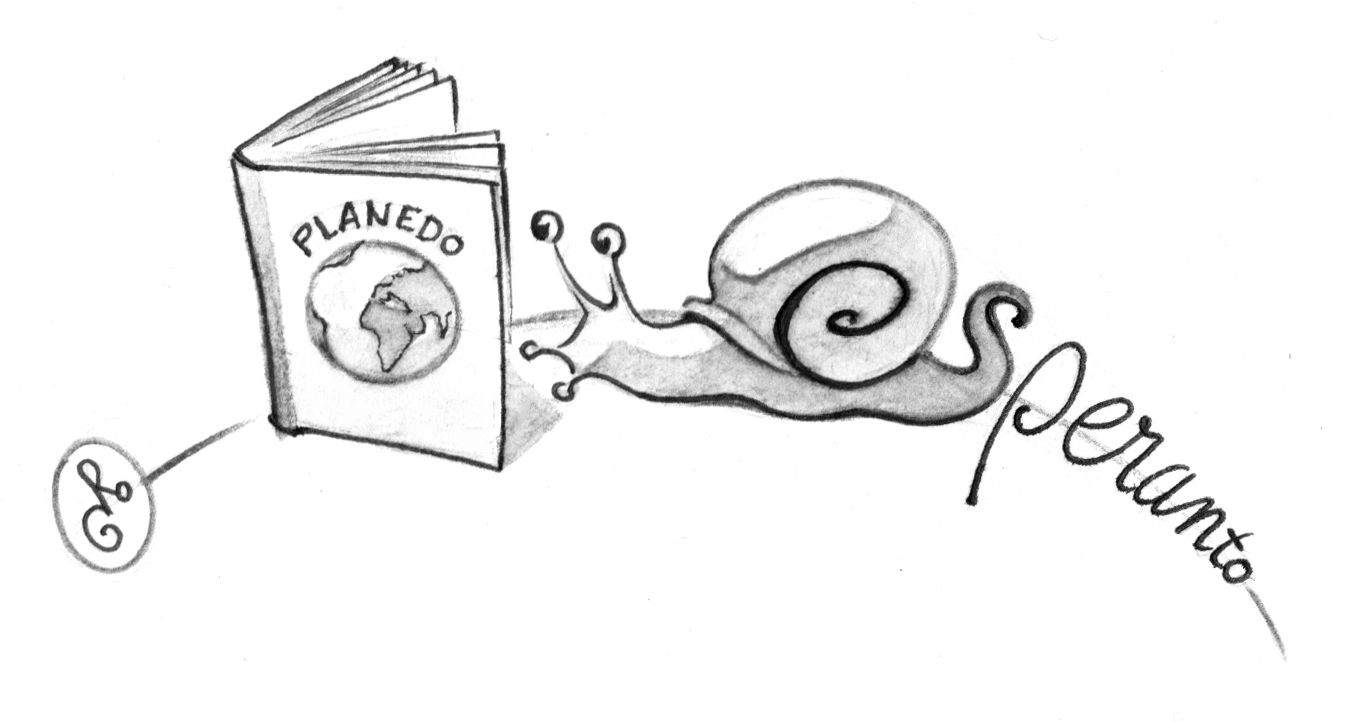
\includegraphics[width=\textwidth]{img/PS_2017_2_heliko.jpg}
\end{figure}

    
{
  \titleformat{\section}[block]{}{}{0pt}{\centering\huge\textbf}
  \titlespacing{\section}{0pt}{4em}{1em}
  \titleformat{\subsection}[block]{}{}{0pt}{\large\textbf}
  \titlespacing{\subsection}{0pt}{2em}{1em}
  \titleformat{\subsubsection}[block]{}{}{0pt}{\small\textbf}
  \titlespacing{\subsubsection}{0pt}{0pt}{0pt}
  \hyphenpenalty=10000\relax  % No hyphenation

  
    \thispagestyle{empty}
    \part*{Adresoj}
  

  

  
    {{ country.grouper.name|cmd:"section" }}
      \vspace{.6em}\nopagebreak
      
        
            {\small
            {\semibold
                Landa OrganizantoLandaj Organizantoj
            }\nopagebreak
            
                {{ profile|full_name }}
                {{ profile.email|escape_latex|cmd:"texttt"|ctx:"footnotesize" }}
            
            }
        \vspace{.7em}
        
      

      
      
        {{ region.grouper|safe|cmd:"subsection*" }}{# TODO: display region's Esperanto or latin name #}
        
          {{ city.grouper|safe|cmd:"subsubsection" }}
            
              \begin{minipage}{\textwidth} {# Address block won't break with minipage #}
              {\small
                {{ place.owner.get_title_display|ctx:"light" }}{# TODO: display also the gender; show only non-deleted (and non-hidden) family members. #}
                {{ place.owner|full_name }}~{{ place.owner.birth_date.year|bracket|ctx:"light" }}, {{ member.first_name }}~{{ member.birth_date.year|bracket|ctx:"light" }}:
                  {{ place.get_postcode_display|escape_latex }}~{{ place.city|escape_latex|ctx:"semibold" }}
                  {{ place.address|escape_latex }} {# TODO: show non-deleted phone numbers according to visibility settings and sorted by importance. #}
                  {{ phone.latex }} {{ phone.comments|escape_latex|ctx:"lightitalic,footnotesize" }} 
                {{ place.owner.email|escape_latex|cmd:"texttt"|ctx:"footnotesize" }}
                  {{ place.max_guest }}g\,\,{{ place.max_night }}n\,\,{{ place.contact_before }}t
                  {{ place.short_description|escape_latex|cmd:"light" }}
                {{ place.conditions.all|join:" " }}
              }
              \vspace{.5em}
              \end{minipage}
            
          
      
      
        
      
  

}

    \ifodd\value{page}\blankpage\fi
\thispagestyle{empty}

\begin{figure}[p]
    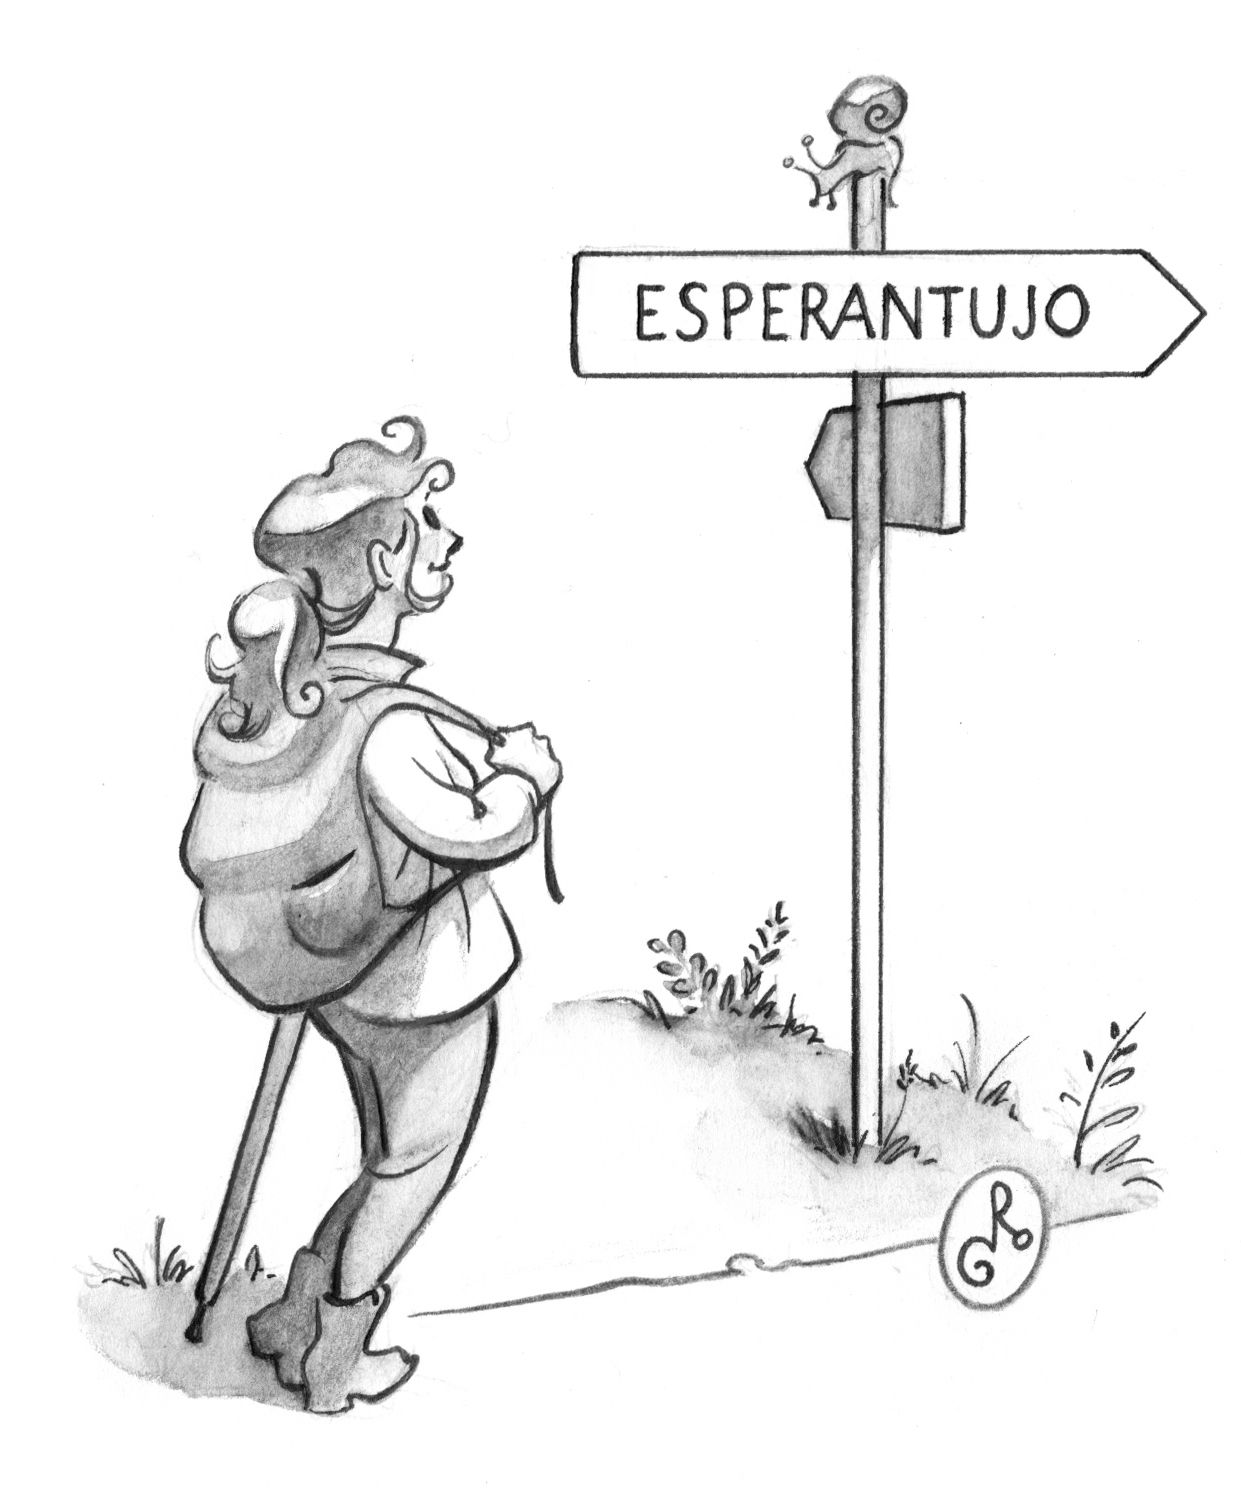
\includegraphics[width=\textwidth]{img/PS_2017_3_tabulo.jpg}
\end{figure}

    \thispagestyle{empty}
\part*{Mapoj}

\invisiblesection{Monda mapo}
\begin{minipage}{\textwidth} 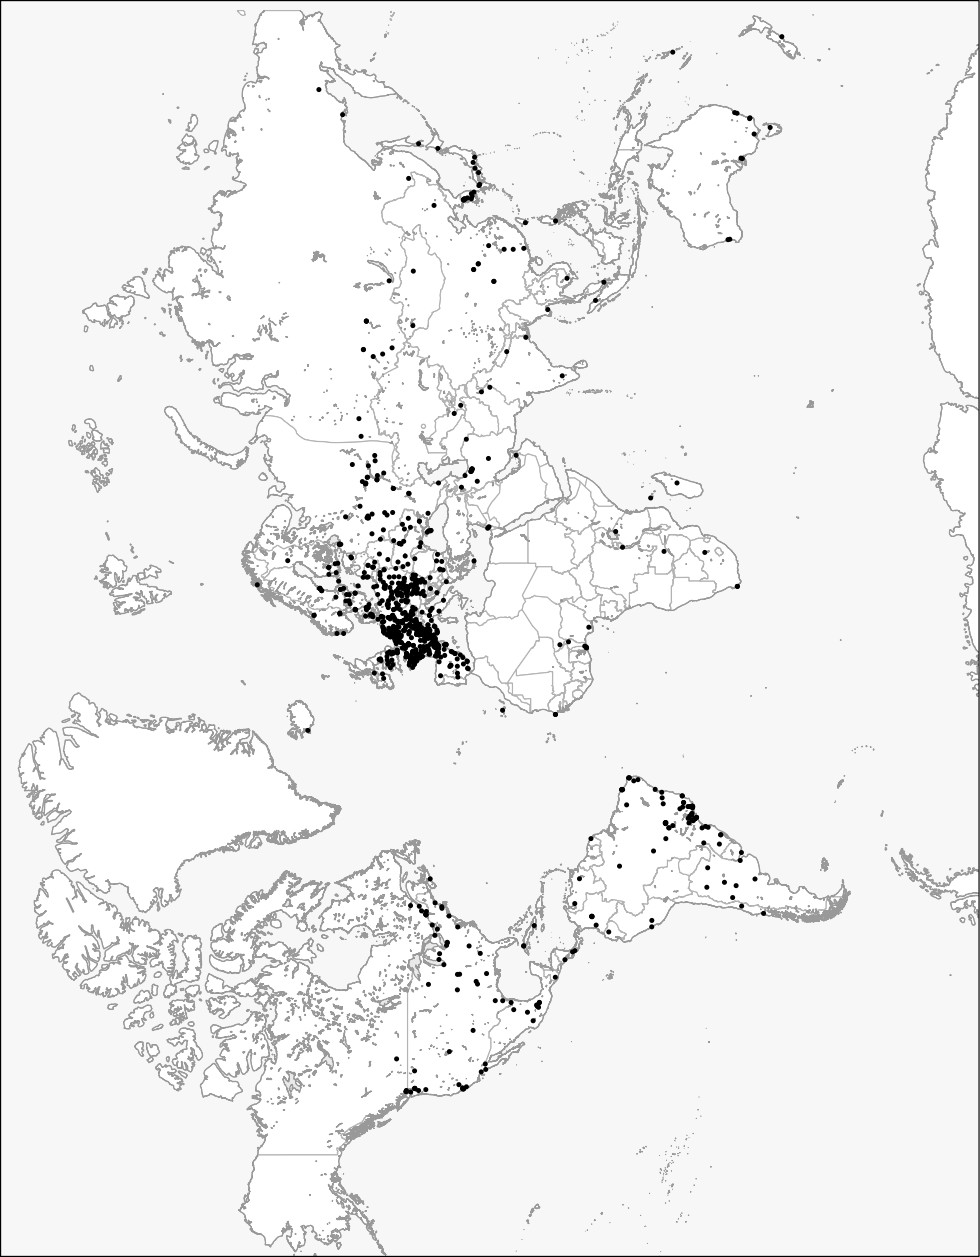
\includegraphics[width=\textwidth]{maps/Mondo.jpg} \end{minipage}

\invisiblesection{Norda Ameriko}
\begin{minipage}{\textwidth} 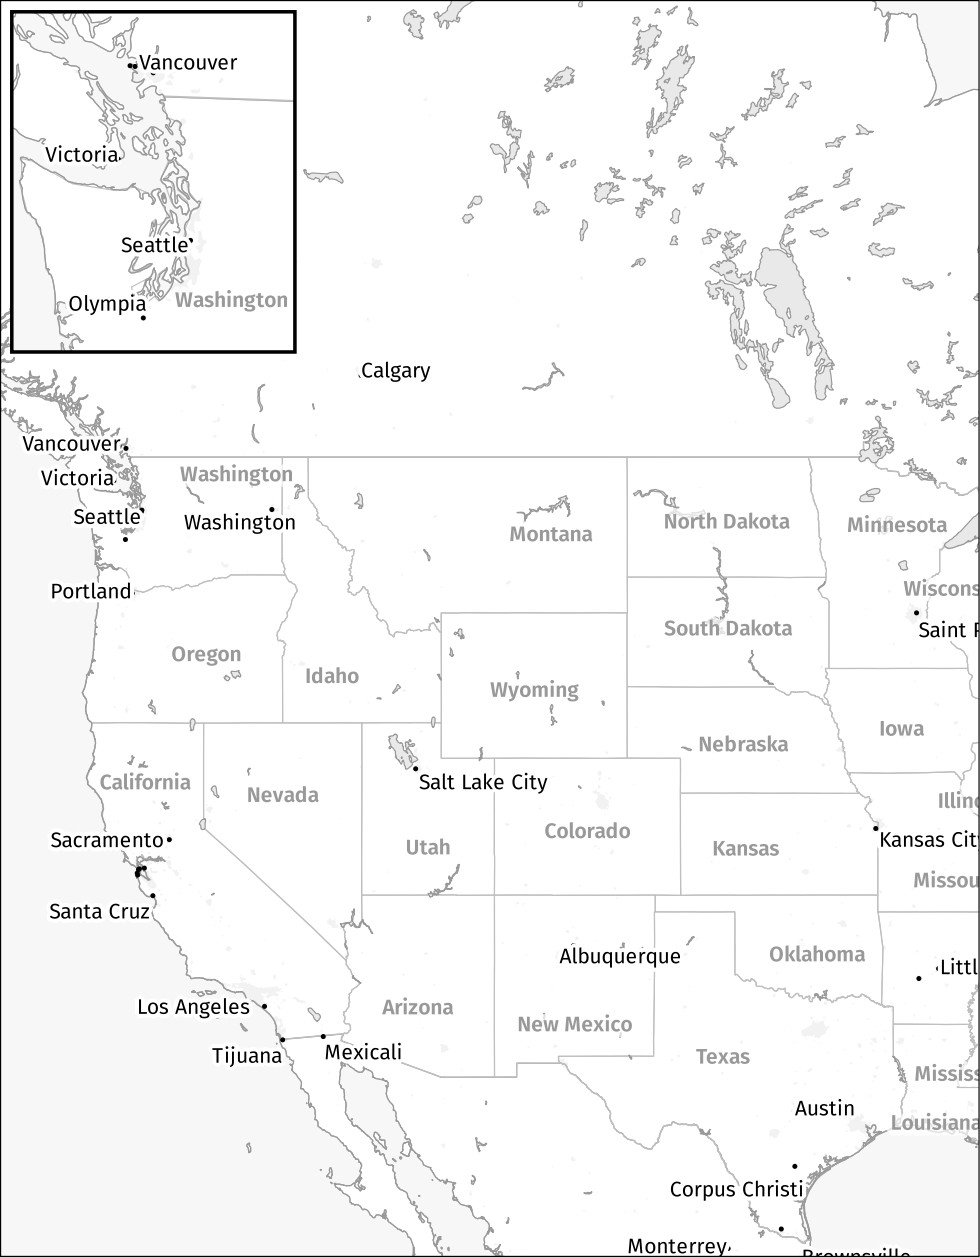
\includegraphics[width=\textwidth]{maps/US.jpg} \end{minipage}
\begin{minipage}{\textwidth}  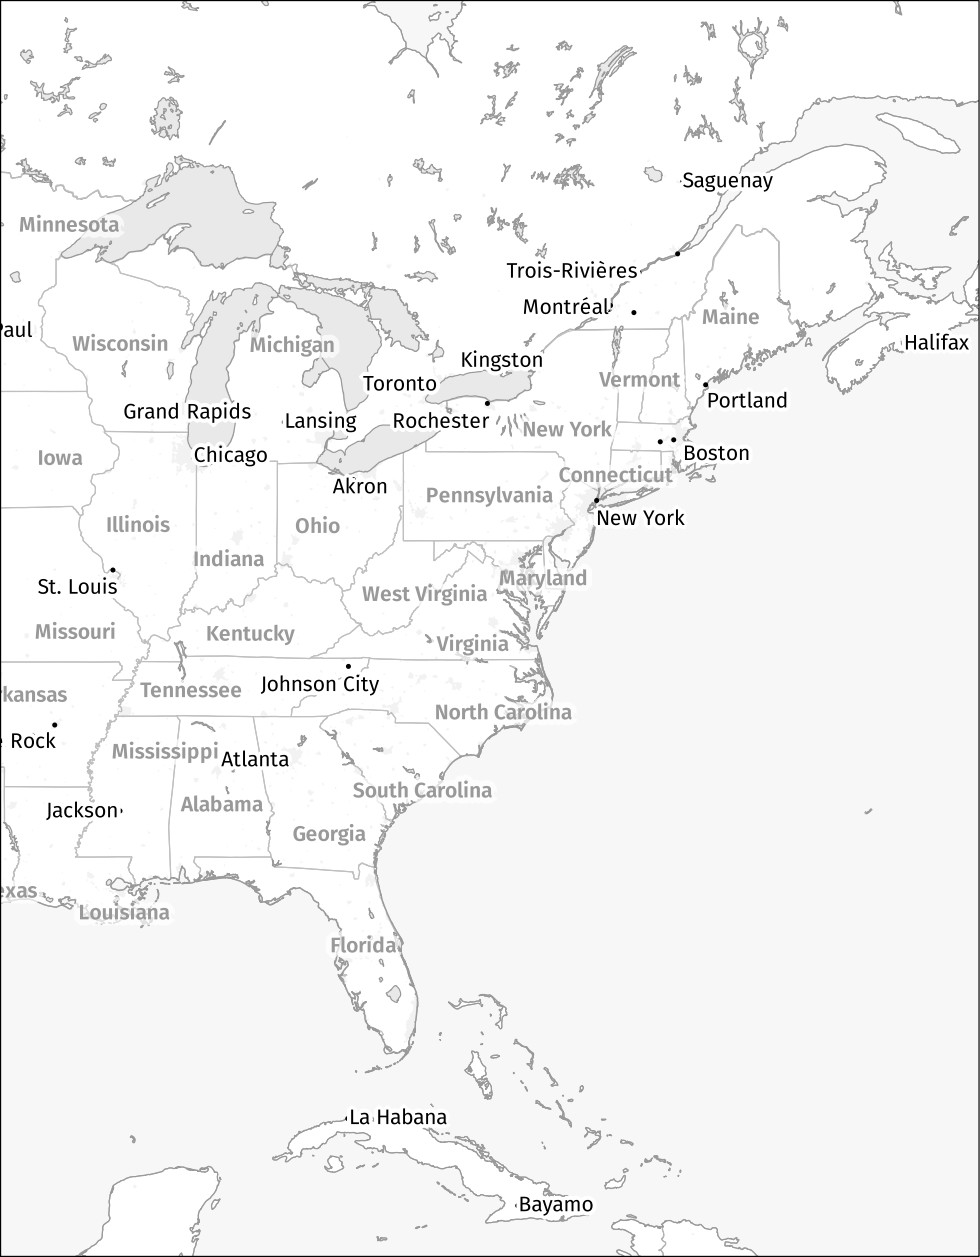
\includegraphics[width=\textwidth]{maps/US_2.jpg} \end{minipage}
\invisiblesection{Suda Ameriko}
\begin{minipage}{\textwidth} 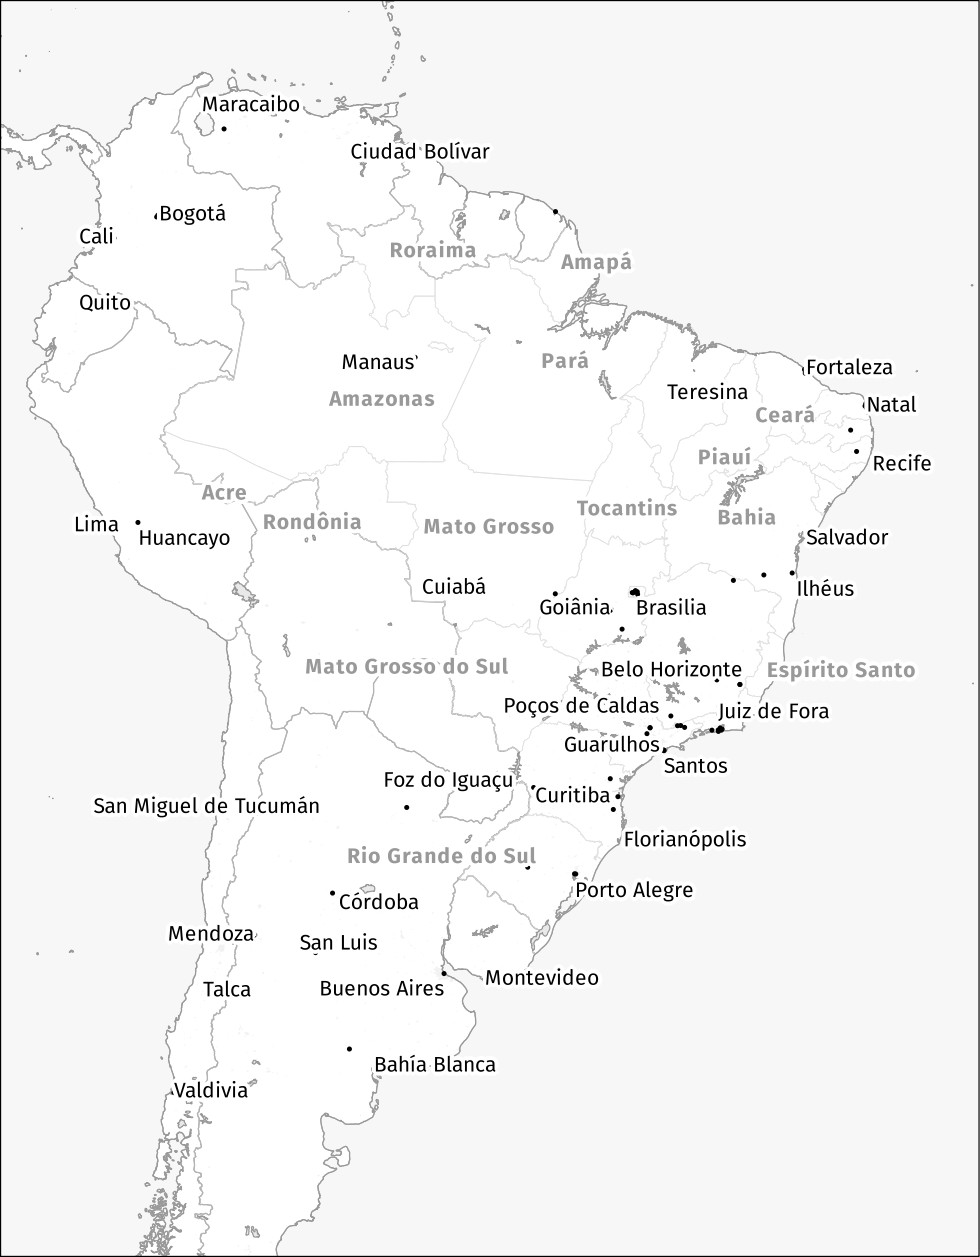
\includegraphics[width=\textwidth]{maps/Ameriko-suda.jpg} \end{minipage}
\invisiblesection{Brazilo}
\begin{minipage}{\textwidth} 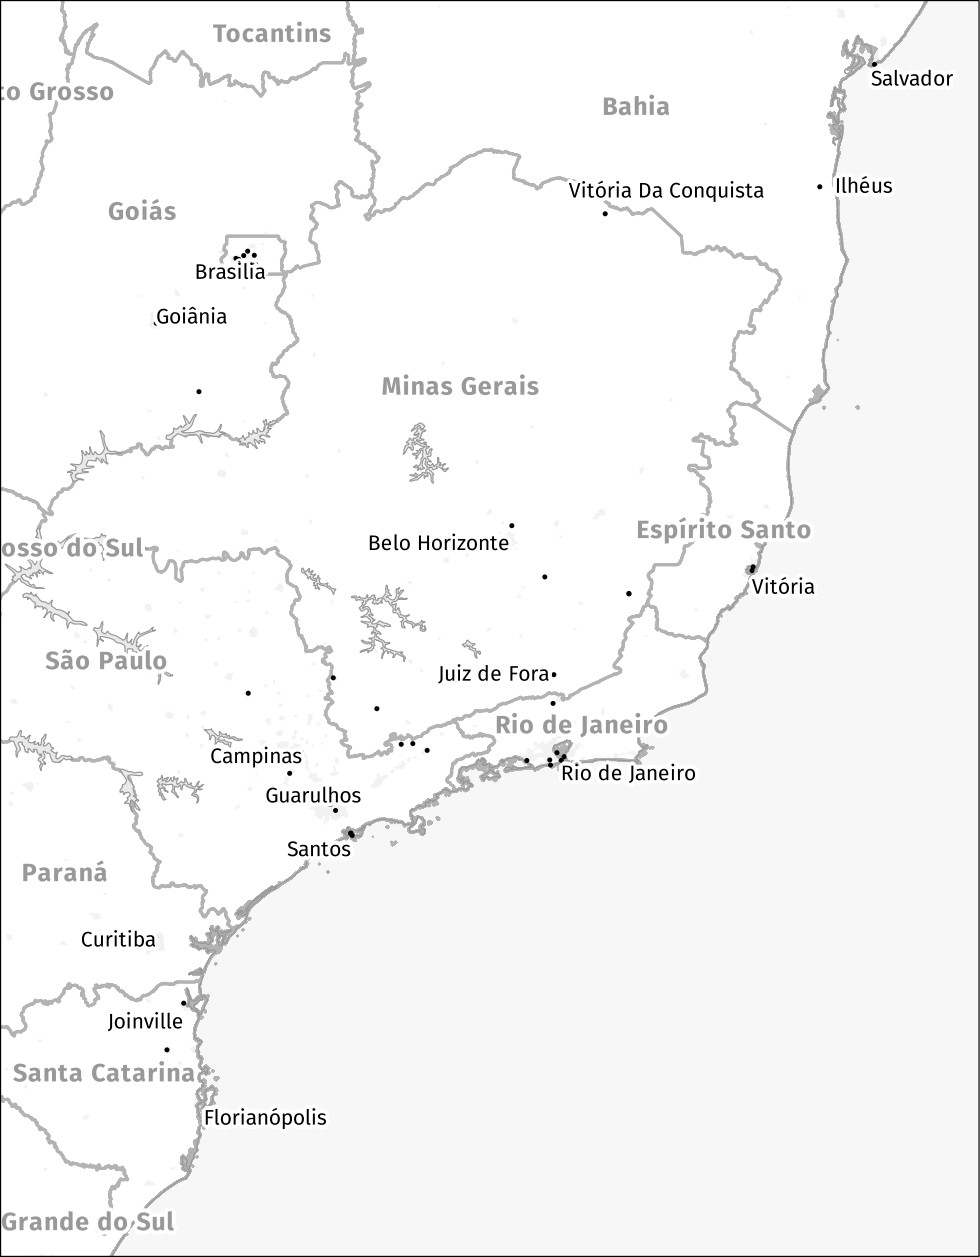
\includegraphics[width=\textwidth]{maps/BR.jpg} \end{minipage}
\invisiblesection{Centra Ameriko}
\begin{minipage}{\textwidth} 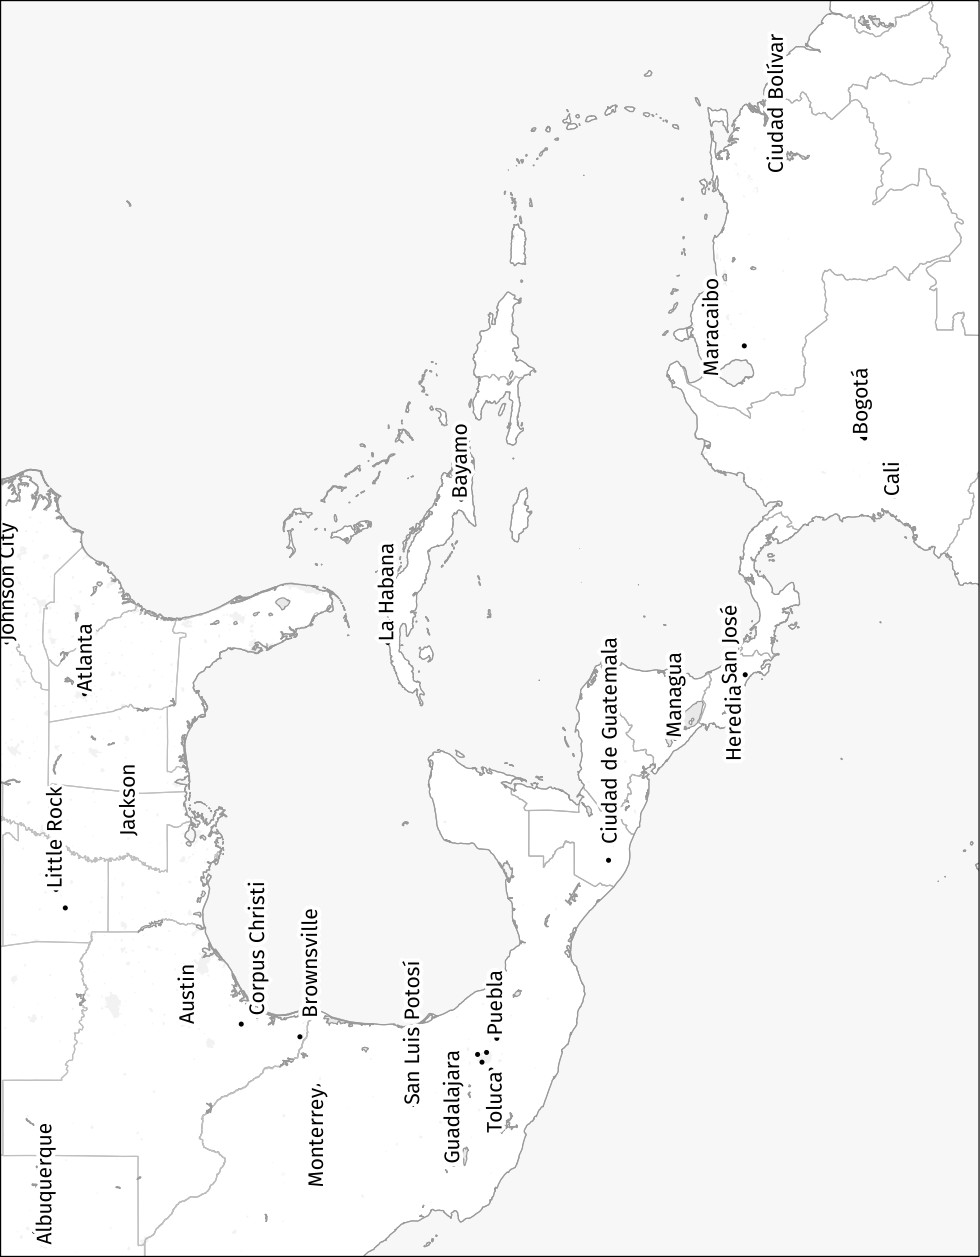
\includegraphics[width=\textwidth]{maps/Ameriko-centra.jpg} \end{minipage}
\invisiblesection{Afriko}
\begin{minipage}{\textwidth} 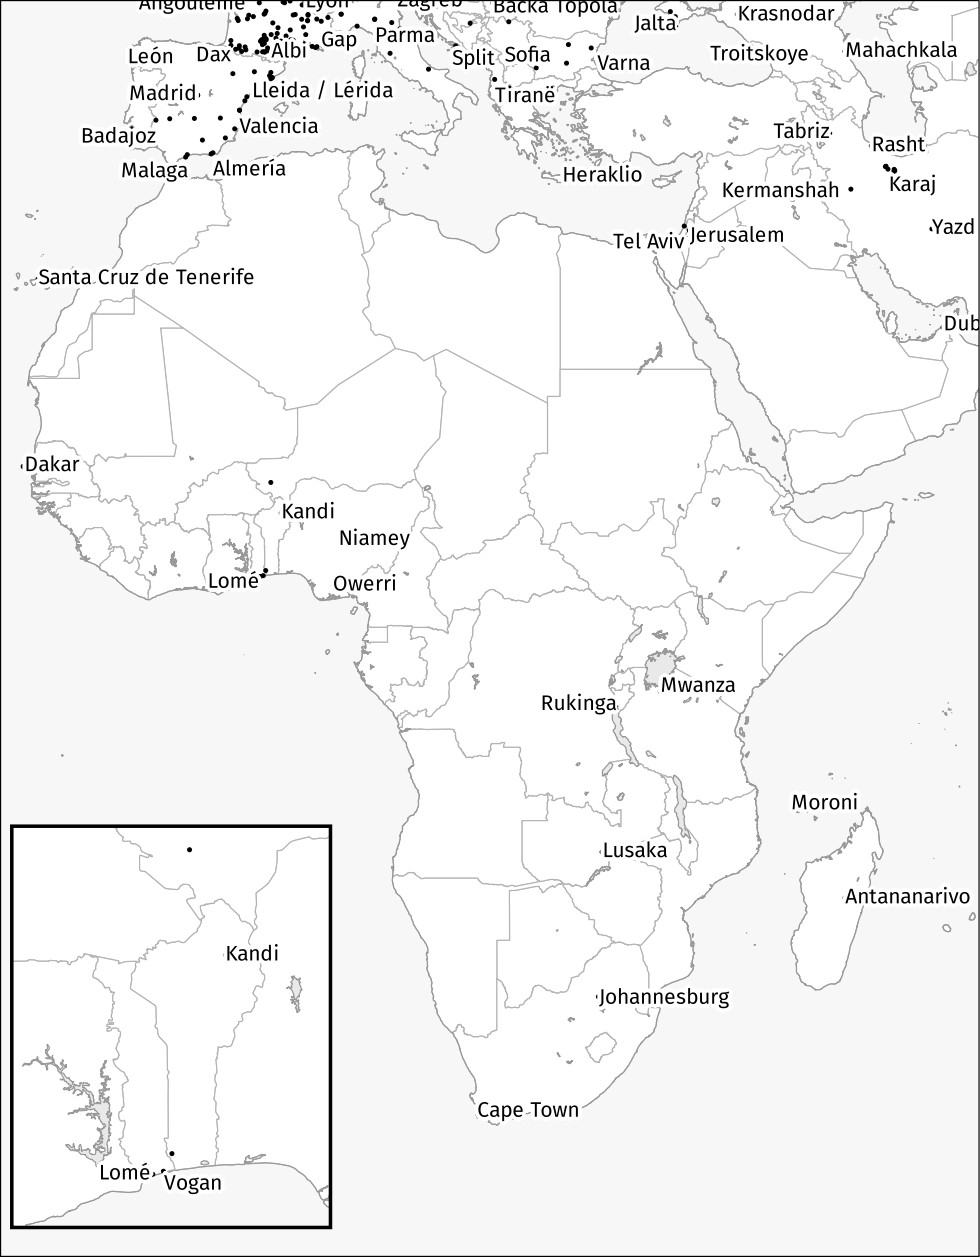
\includegraphics[width=\textwidth]{maps/Afriko.jpg} \end{minipage}

\invisiblesection{Eŭropo}
\begin{minipage}{\textwidth} 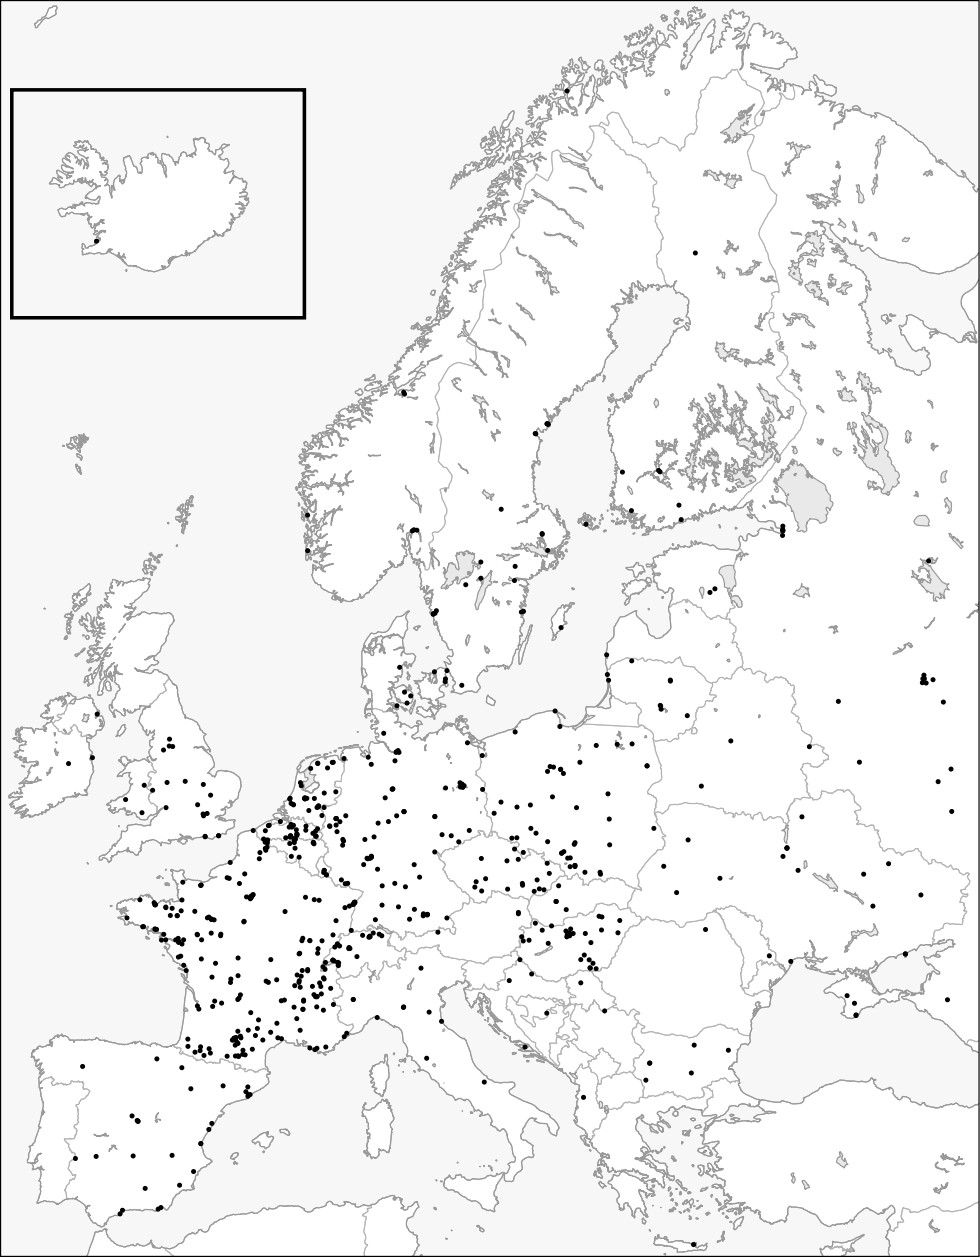
\includegraphics[width=\textwidth]{maps/Europo.jpg} \end{minipage}
\invisiblesection{Norda Eŭropo}
\begin{minipage}{\textwidth} 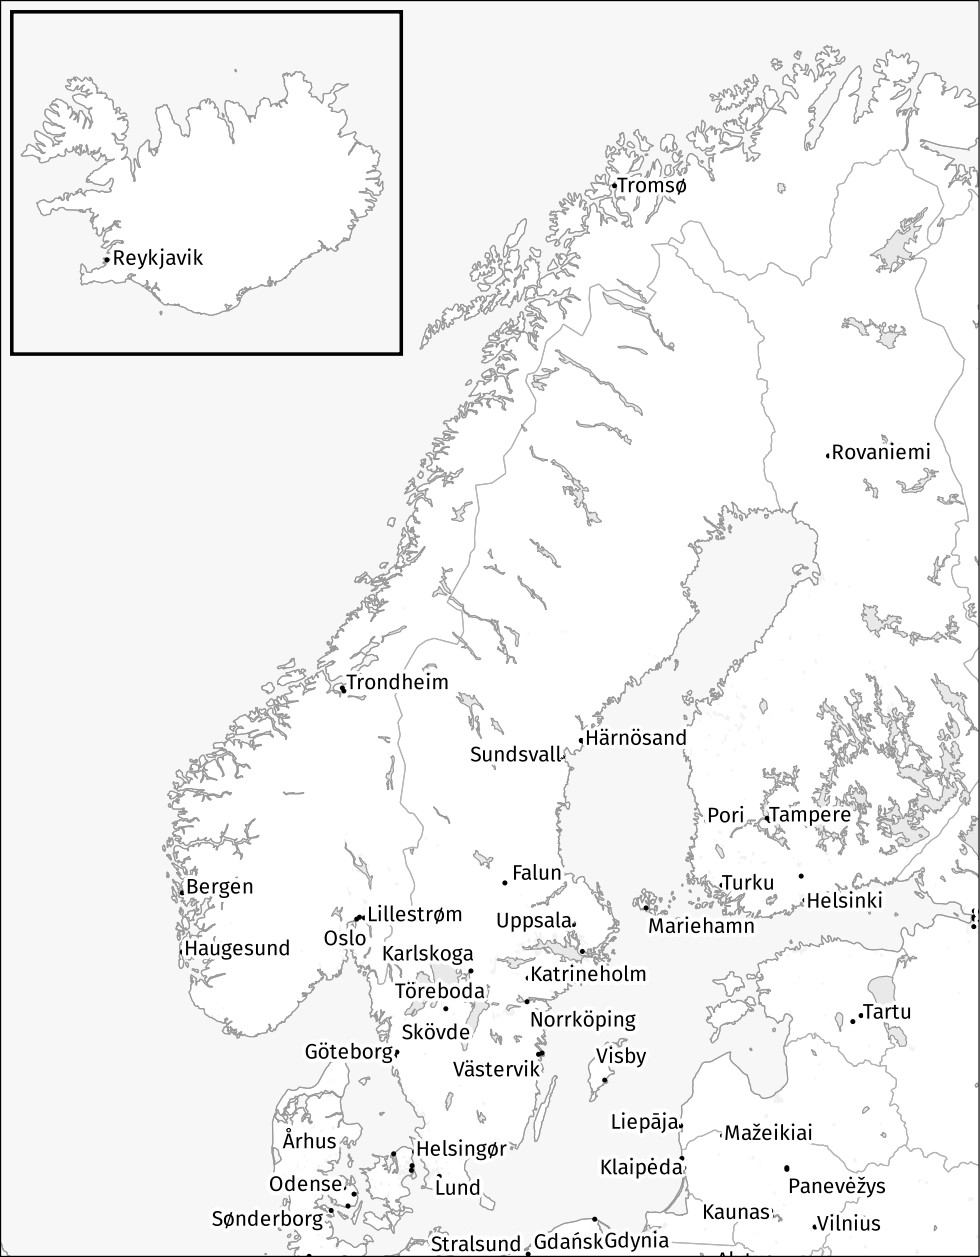
\includegraphics[width=\textwidth]{maps/EU-norda.jpg} \end{minipage}
\invisiblesection{Britio kaj Irlando}
\begin{minipage}{\textwidth} 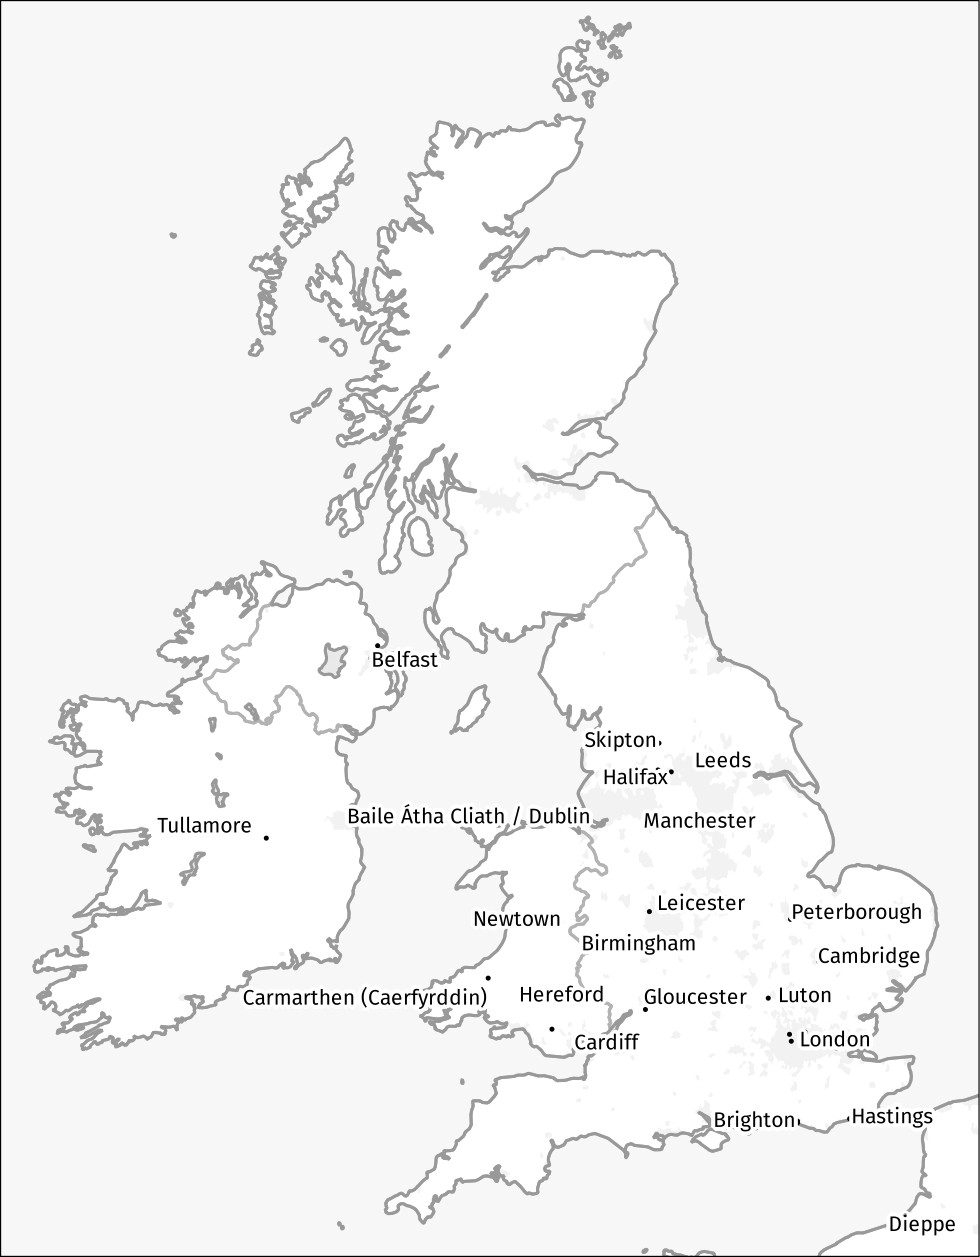
\includegraphics[width=\textwidth]{maps/GB.jpg} \end{minipage}
\invisiblesection{Benelukso}
\begin{minipage}{\textwidth} 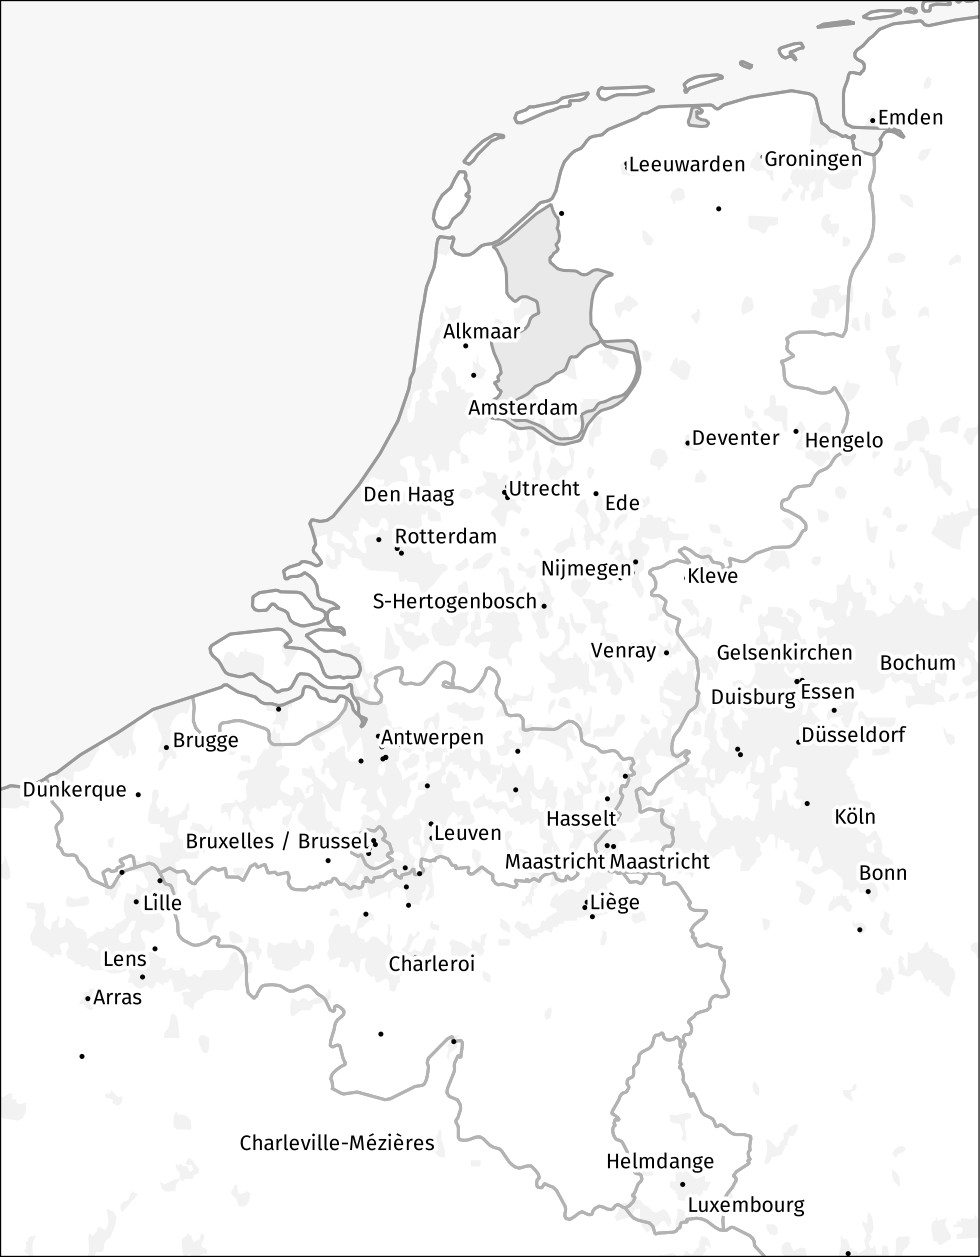
\includegraphics[width=\textwidth]{maps/BENELU.jpg} \end{minipage}
\invisiblesection{Francio}
\begin{minipage}{\textwidth} 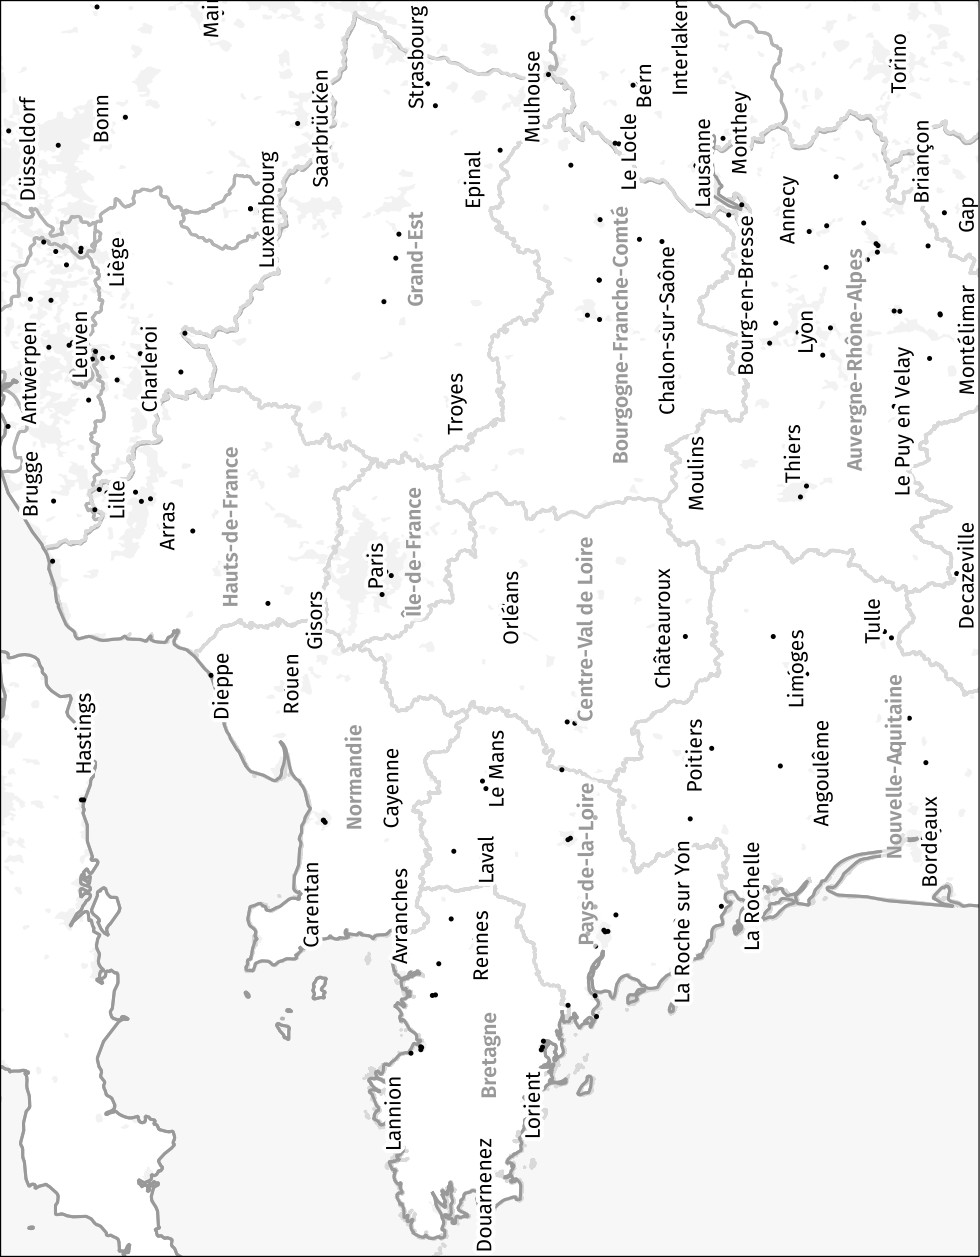
\includegraphics[width=\textwidth]{maps/FR.jpg} \end{minipage}
\begin{minipage}{\textwidth} 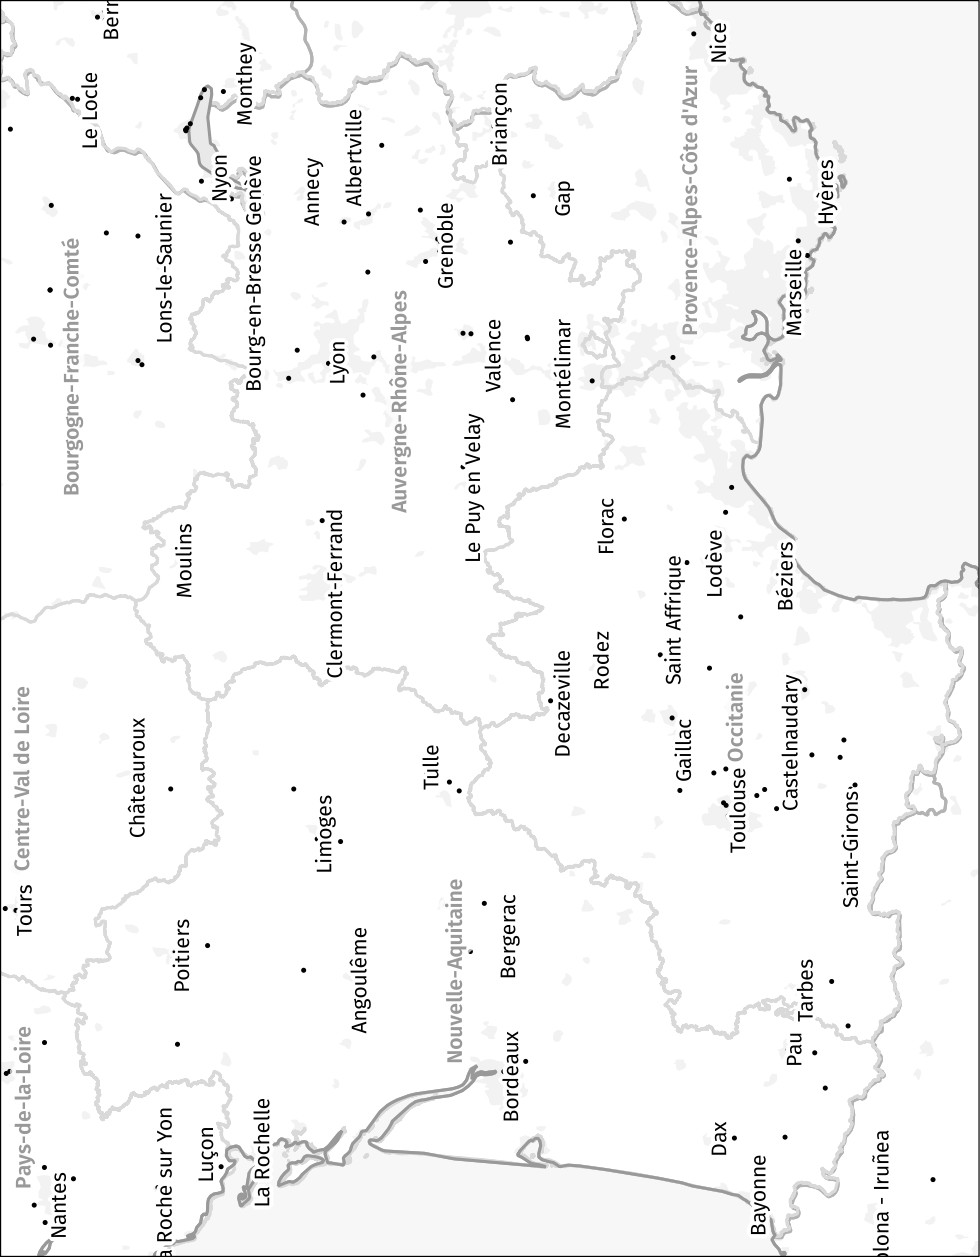
\includegraphics[width=\textwidth]{maps/FR_2.jpg} \end{minipage}
\invisiblesection{Hispanio}
\begin{minipage}{\textwidth} 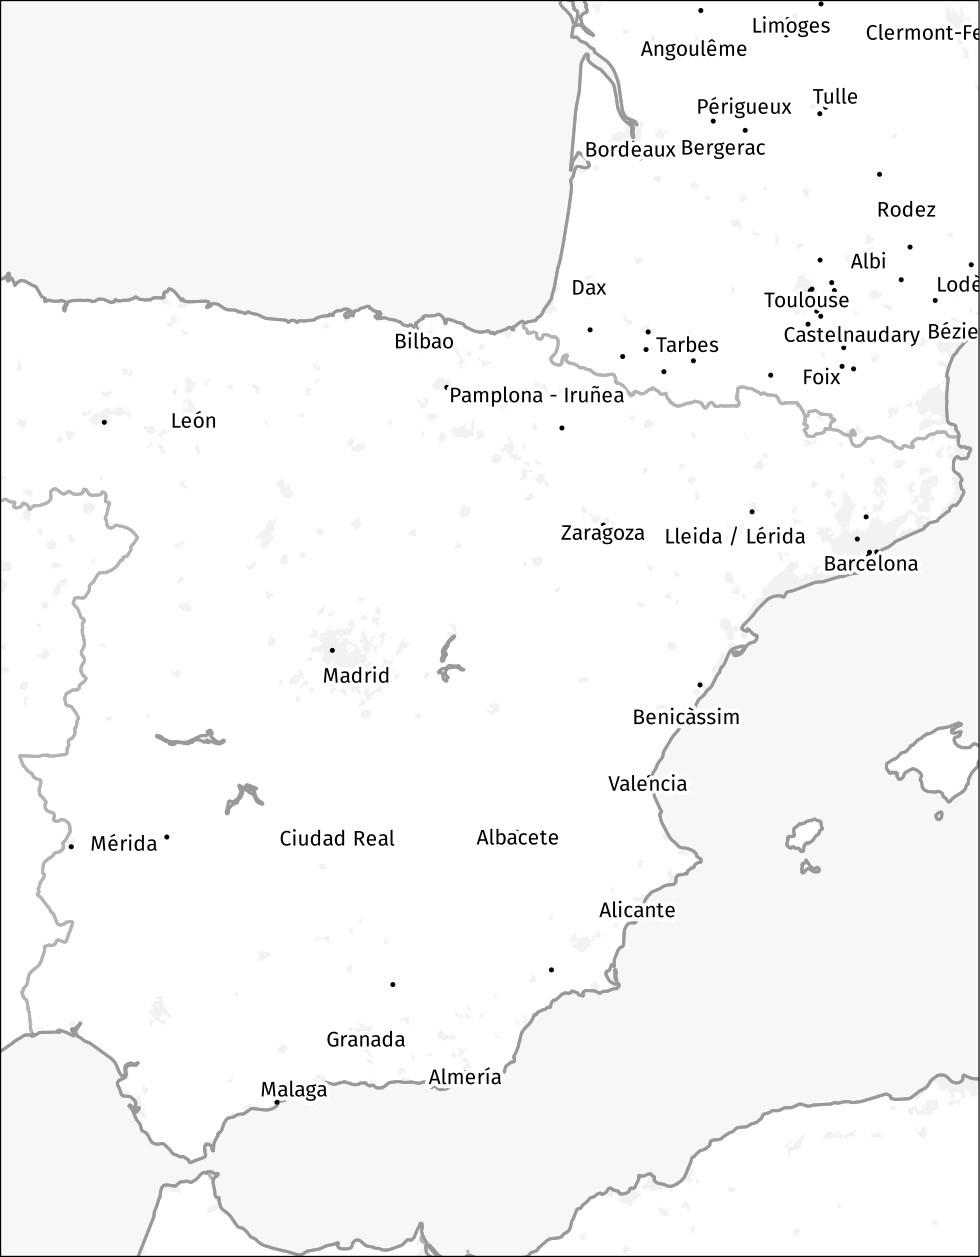
\includegraphics[width=\textwidth]{maps/ES.jpg} \end{minipage}
\invisiblesection{Germanio}
\begin{minipage}{\textwidth} 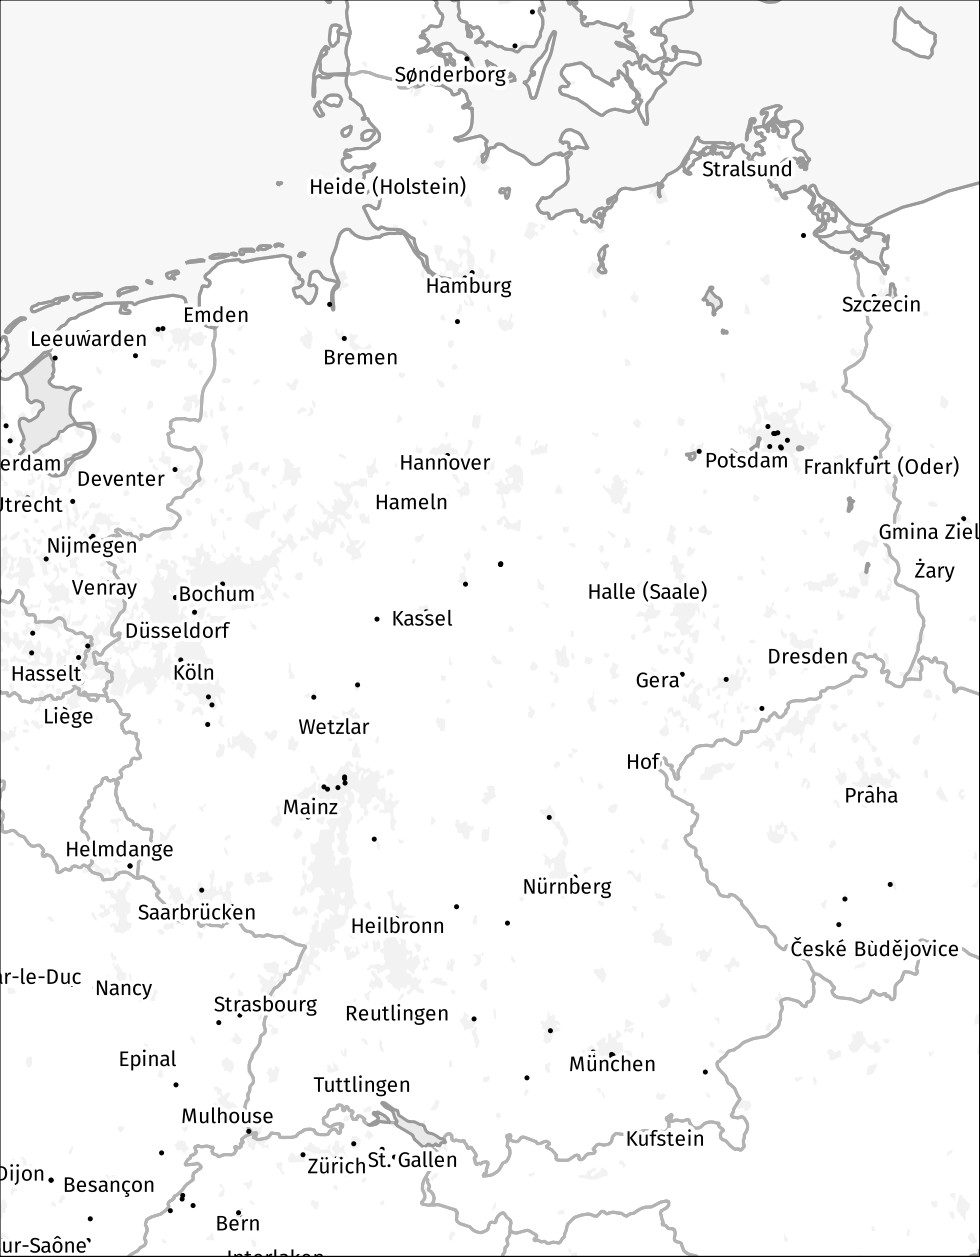
\includegraphics[width=\textwidth]{maps/DE.jpg} \end{minipage}
\invisiblesection{Italio kaj Svislando}
\begin{minipage}{\textwidth} 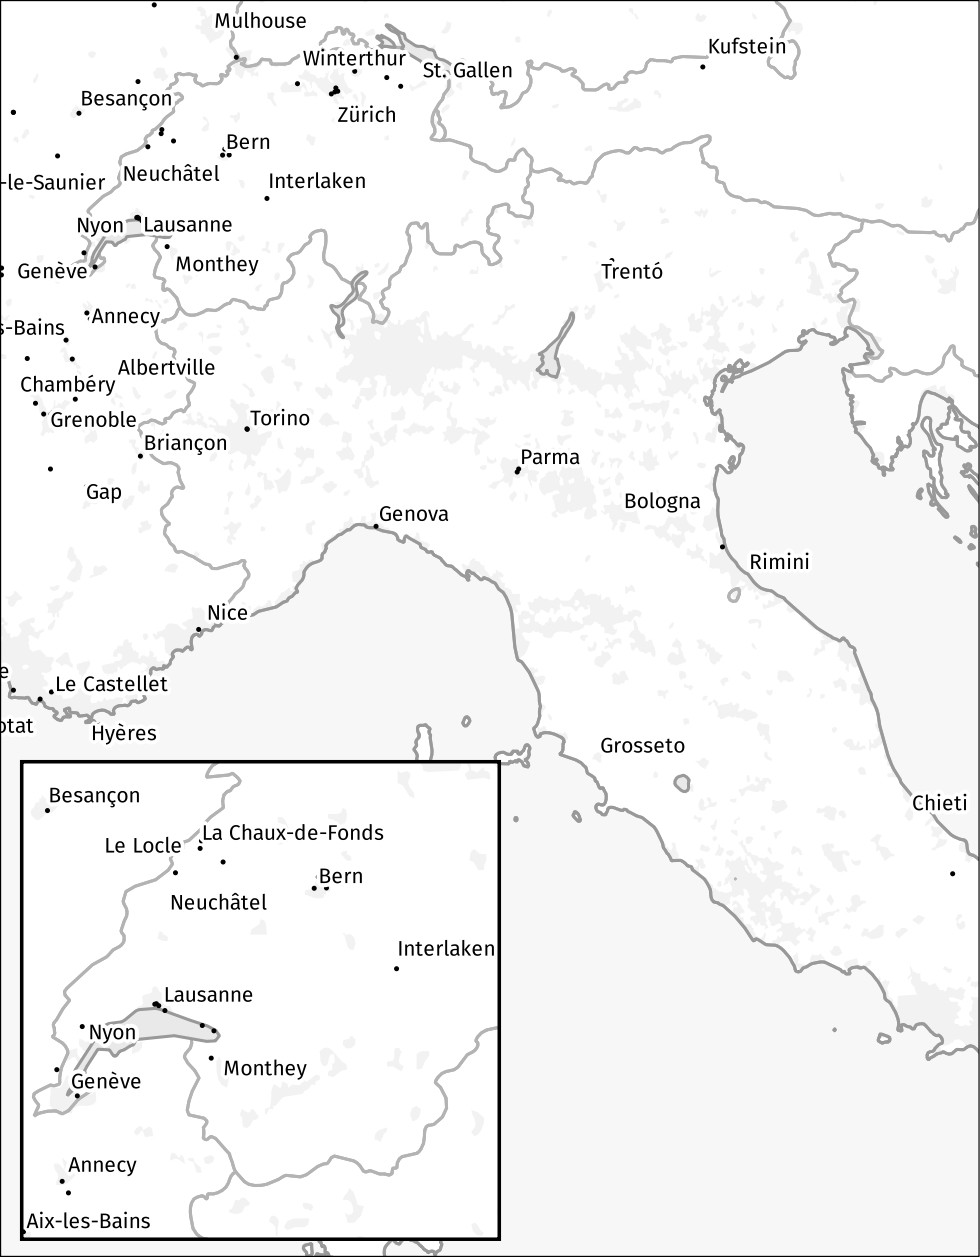
\includegraphics[width=\textwidth]{maps/CH-IT.jpg} \end{minipage}
\invisiblesection{Centra Eŭropo}
\begin{minipage}{\textwidth} 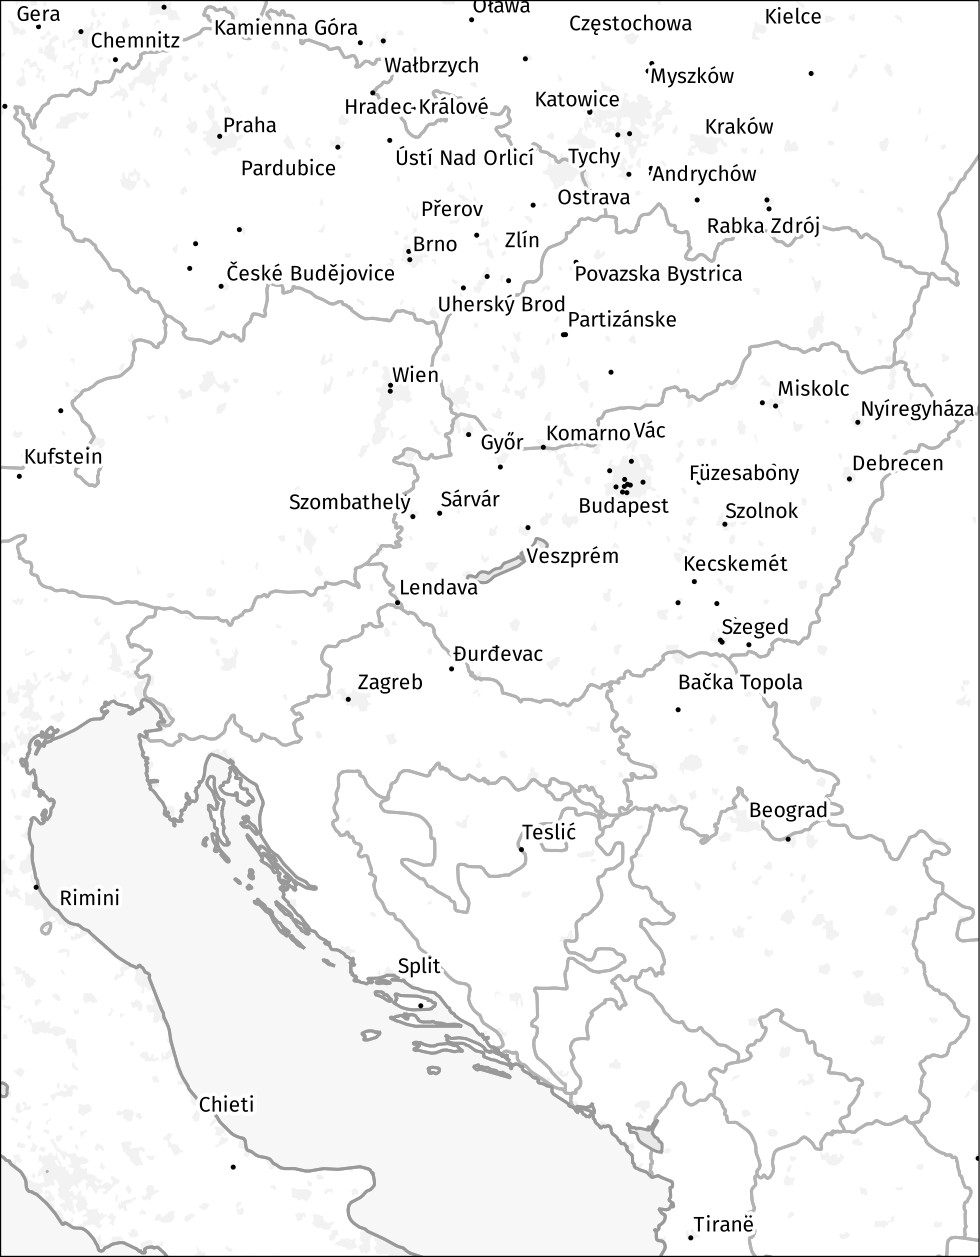
\includegraphics[width=\textwidth]{maps/EU-centra.jpg} \end{minipage}
\invisiblesection{Pollando}
\begin{minipage}{\textwidth} 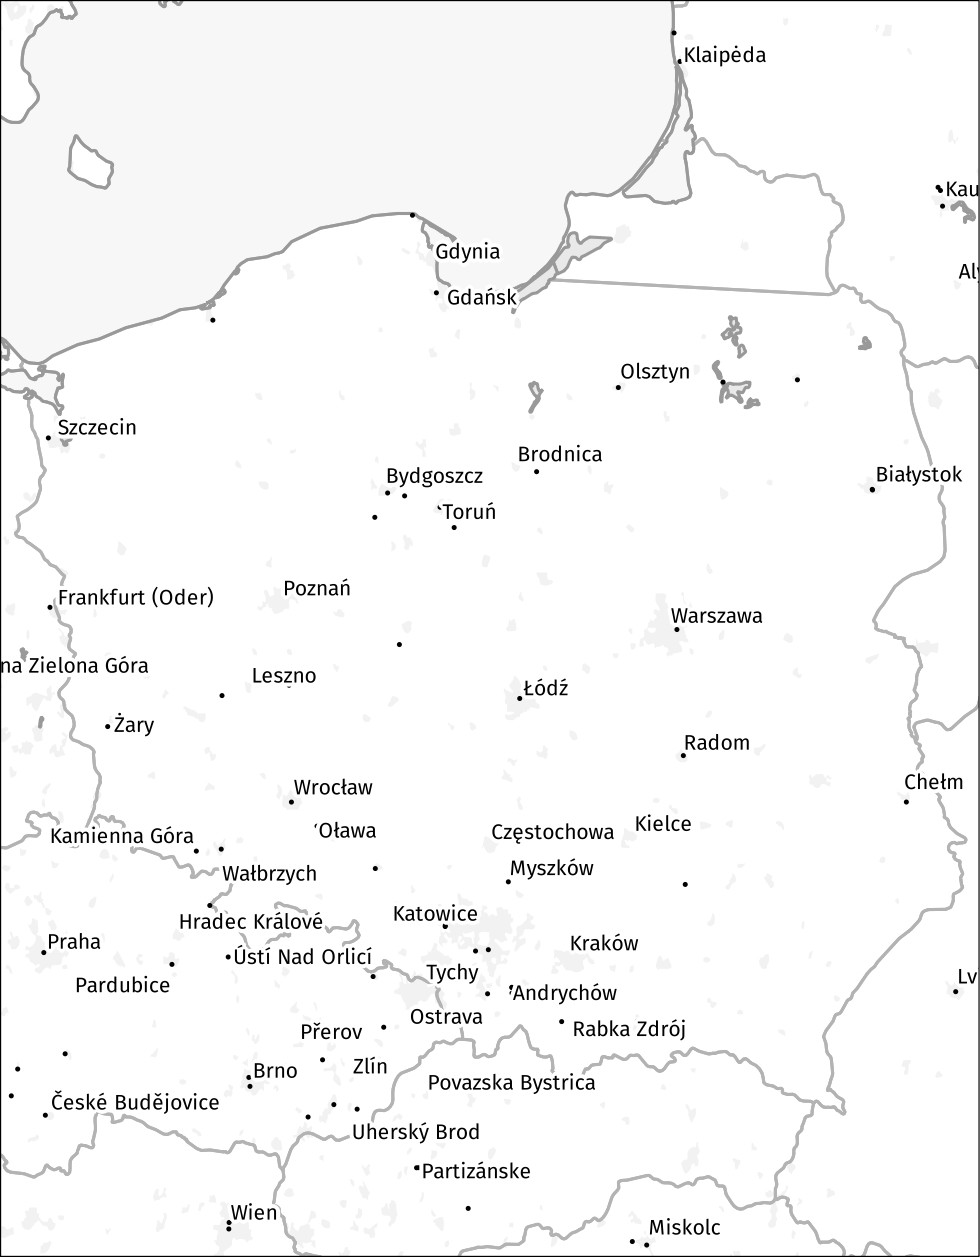
\includegraphics[width=\textwidth]{maps/PL.jpg} \end{minipage}
\invisiblesection{Rusio}
\begin{minipage}{\textwidth} 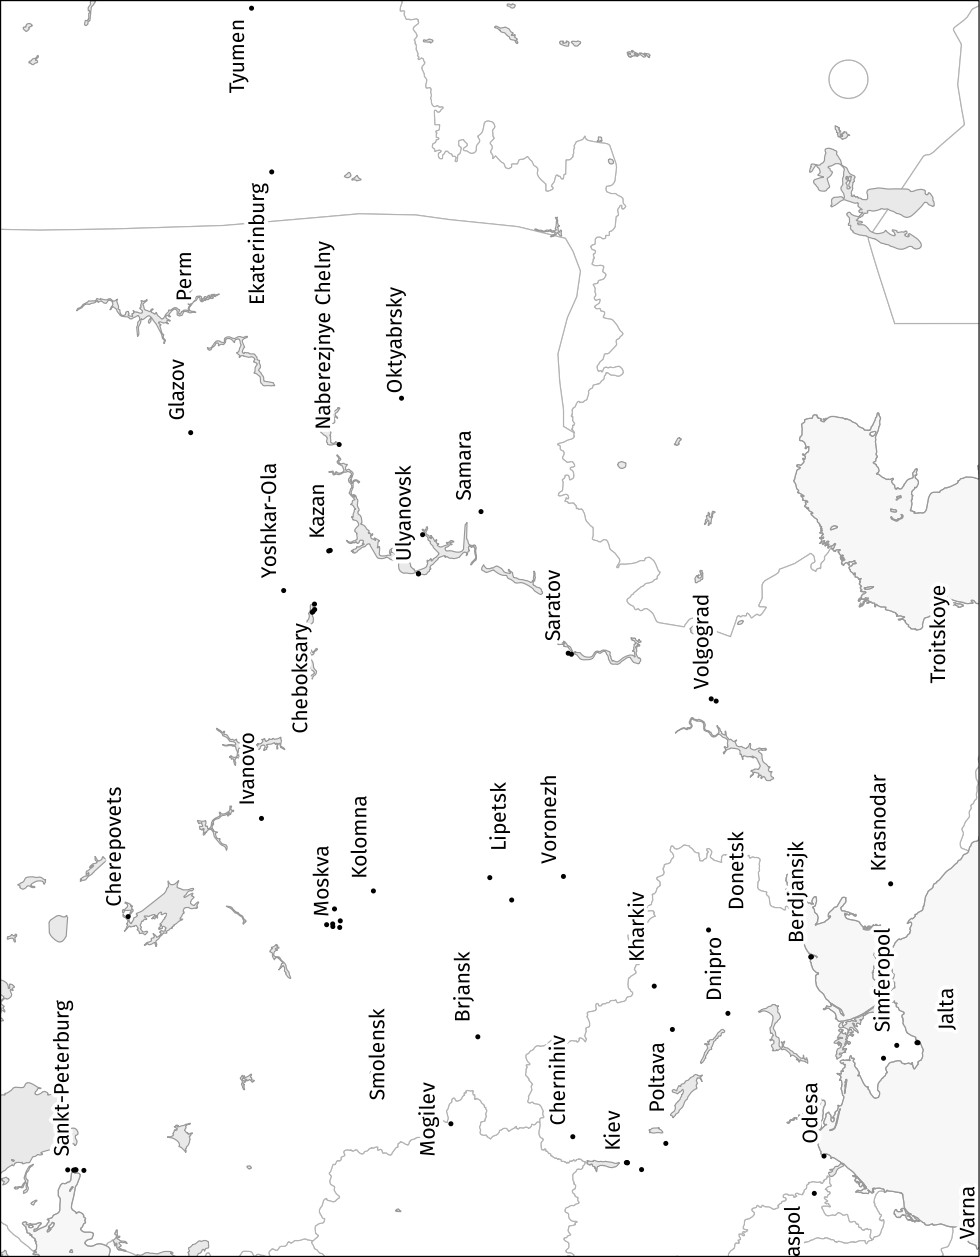
\includegraphics[width=\textwidth]{maps/RU.jpg} \end{minipage}
\invisiblesection{Ukrainio}
\begin{minipage}{\textwidth} 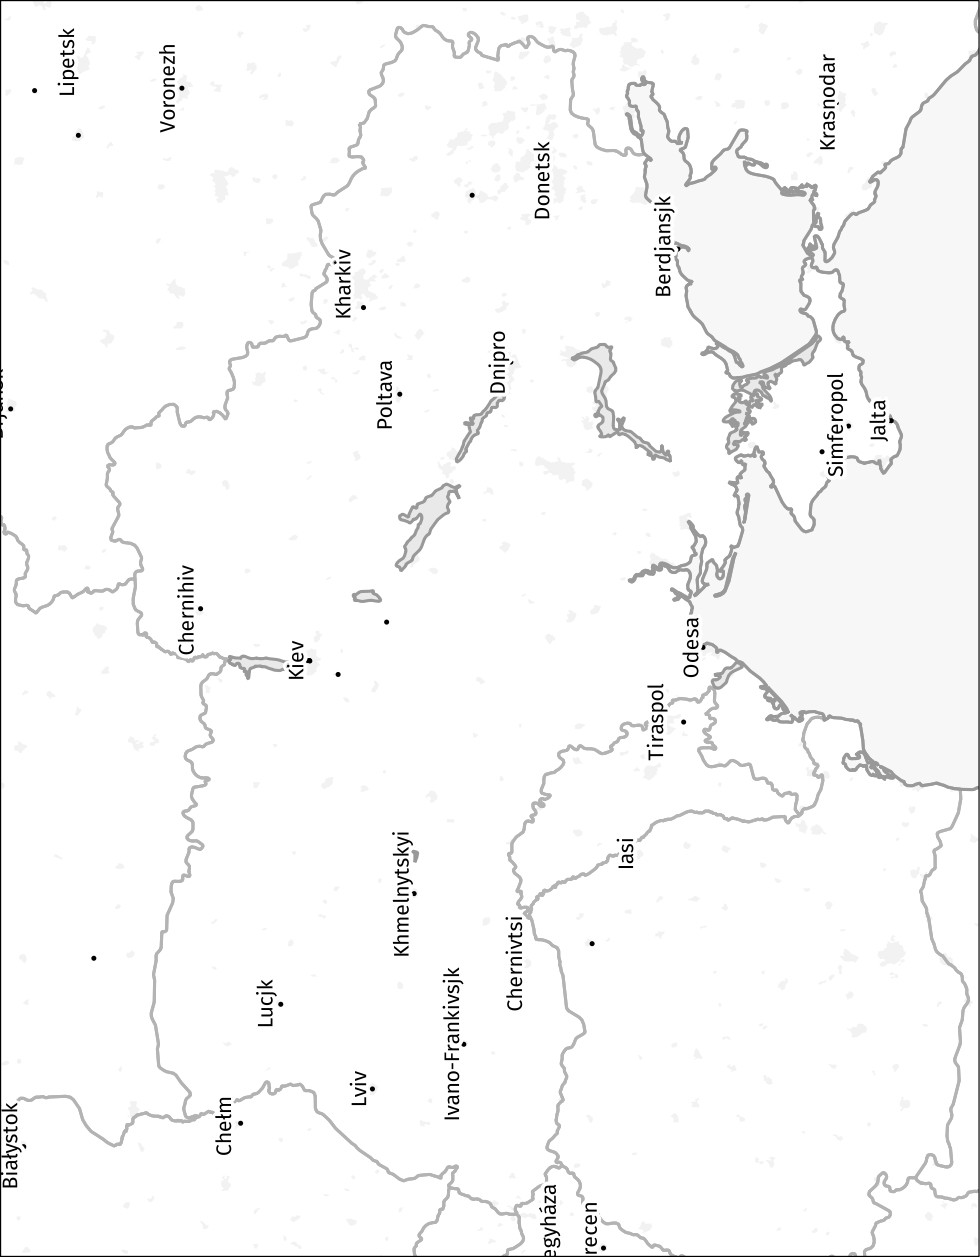
\includegraphics[width=\textwidth]{maps/UA.jpg} \end{minipage}

\invisiblesection{Centra kaj Okcidenta Azio}
\begin{minipage}{\textwidth} 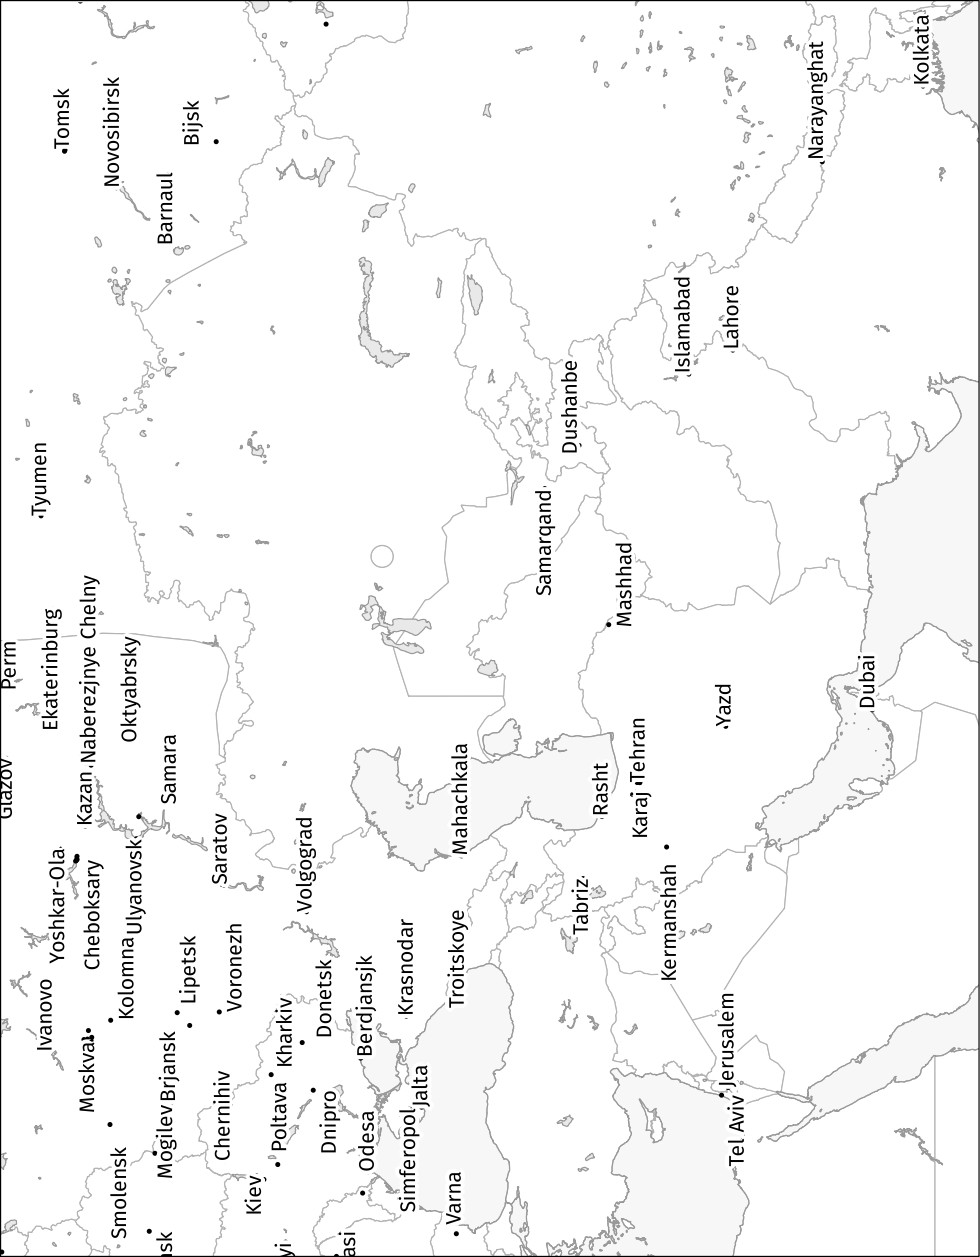
\includegraphics[width=\textwidth]{maps/Azio-centra.jpg} \end{minipage}
\invisiblesection{Azio, orienta parto}
\begin{minipage}{\textwidth} 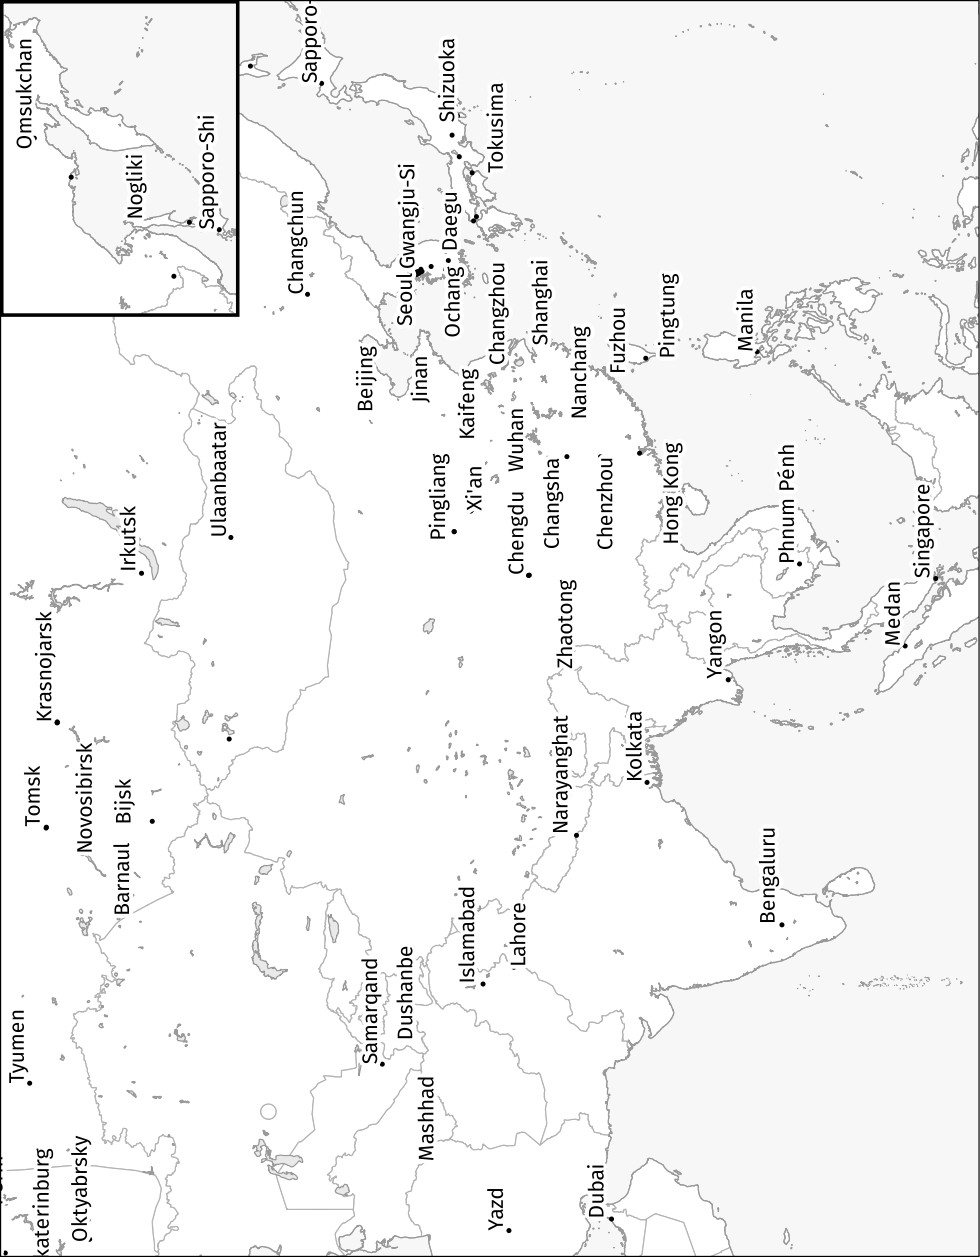
\includegraphics[width=\textwidth]{maps/Azio-orienta.jpg} \end{minipage}
\invisiblesection{Japanio}
\begin{minipage}{\textwidth} 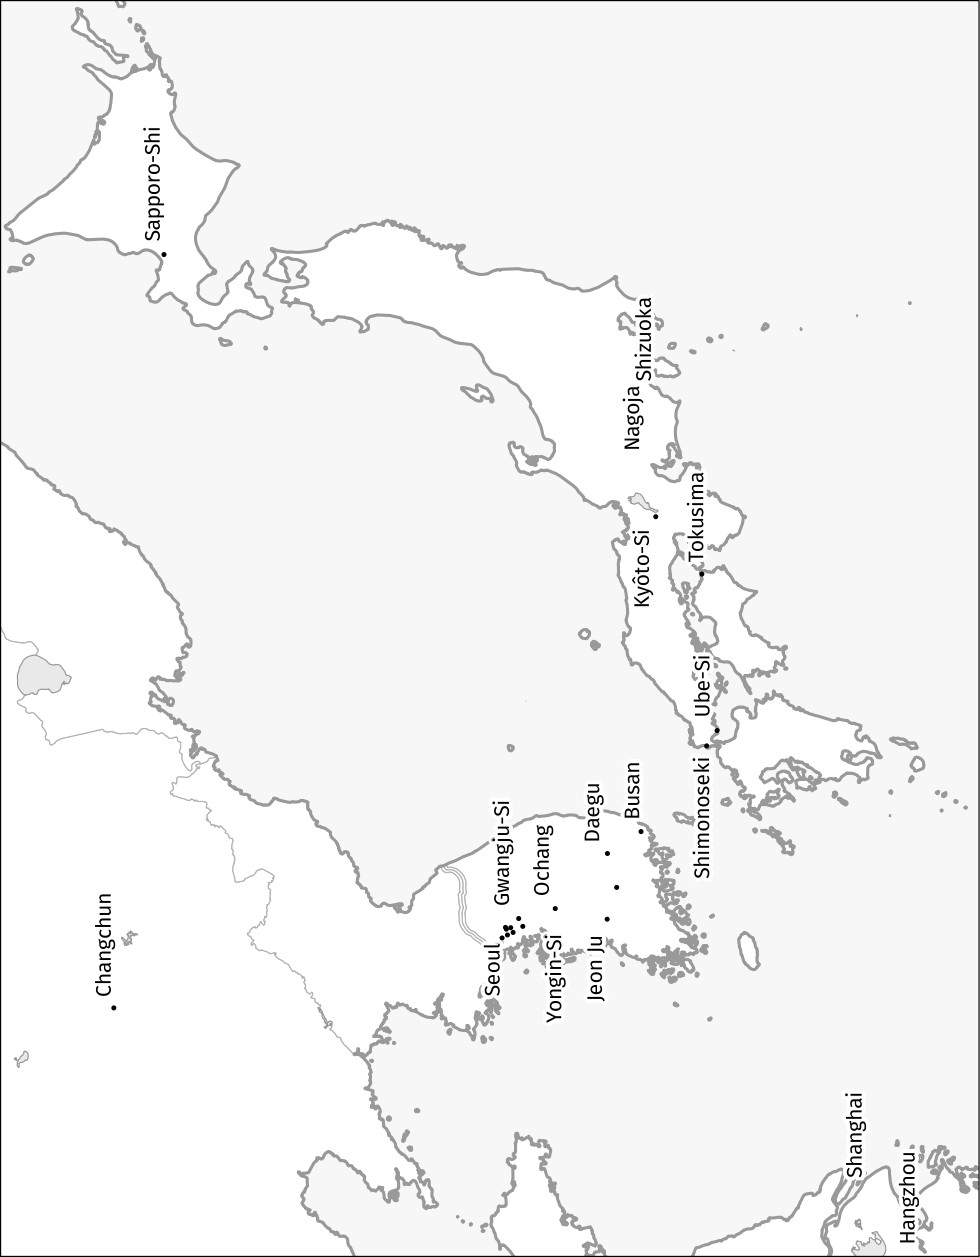
\includegraphics[width=\textwidth]{maps/JP.jpg} \end{minipage}
\invisiblesection{Aŭstralio}
\begin{minipage}{\textwidth} 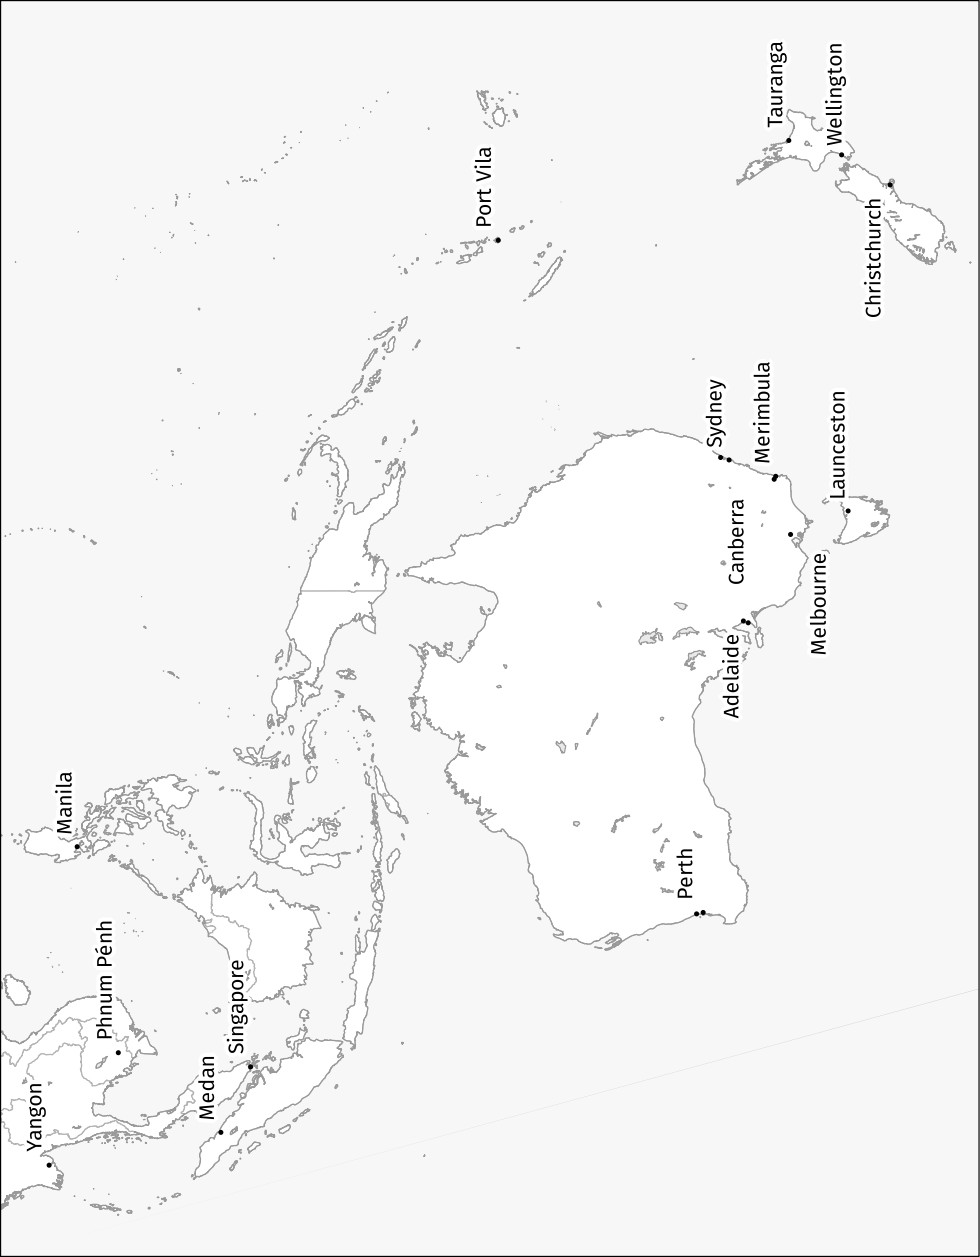
\includegraphics[width=\textwidth]{maps/Oceanio.jpg} \end{minipage}

    \invisiblesection*{Notoj}
\fancyfoot{}
\blankpage

\foreach \i in {1,...,3}{
  \foreach \j in {1,...,13}{
    \vspace{1.1em}
    \textcolor{light-gray}{\hrulefill} \par
  }
  \newpage
}

\blankpage

    \ifodd\value{page}\blankpage\fi
\thispagestyle{empty}

\begin{figure}[p]
    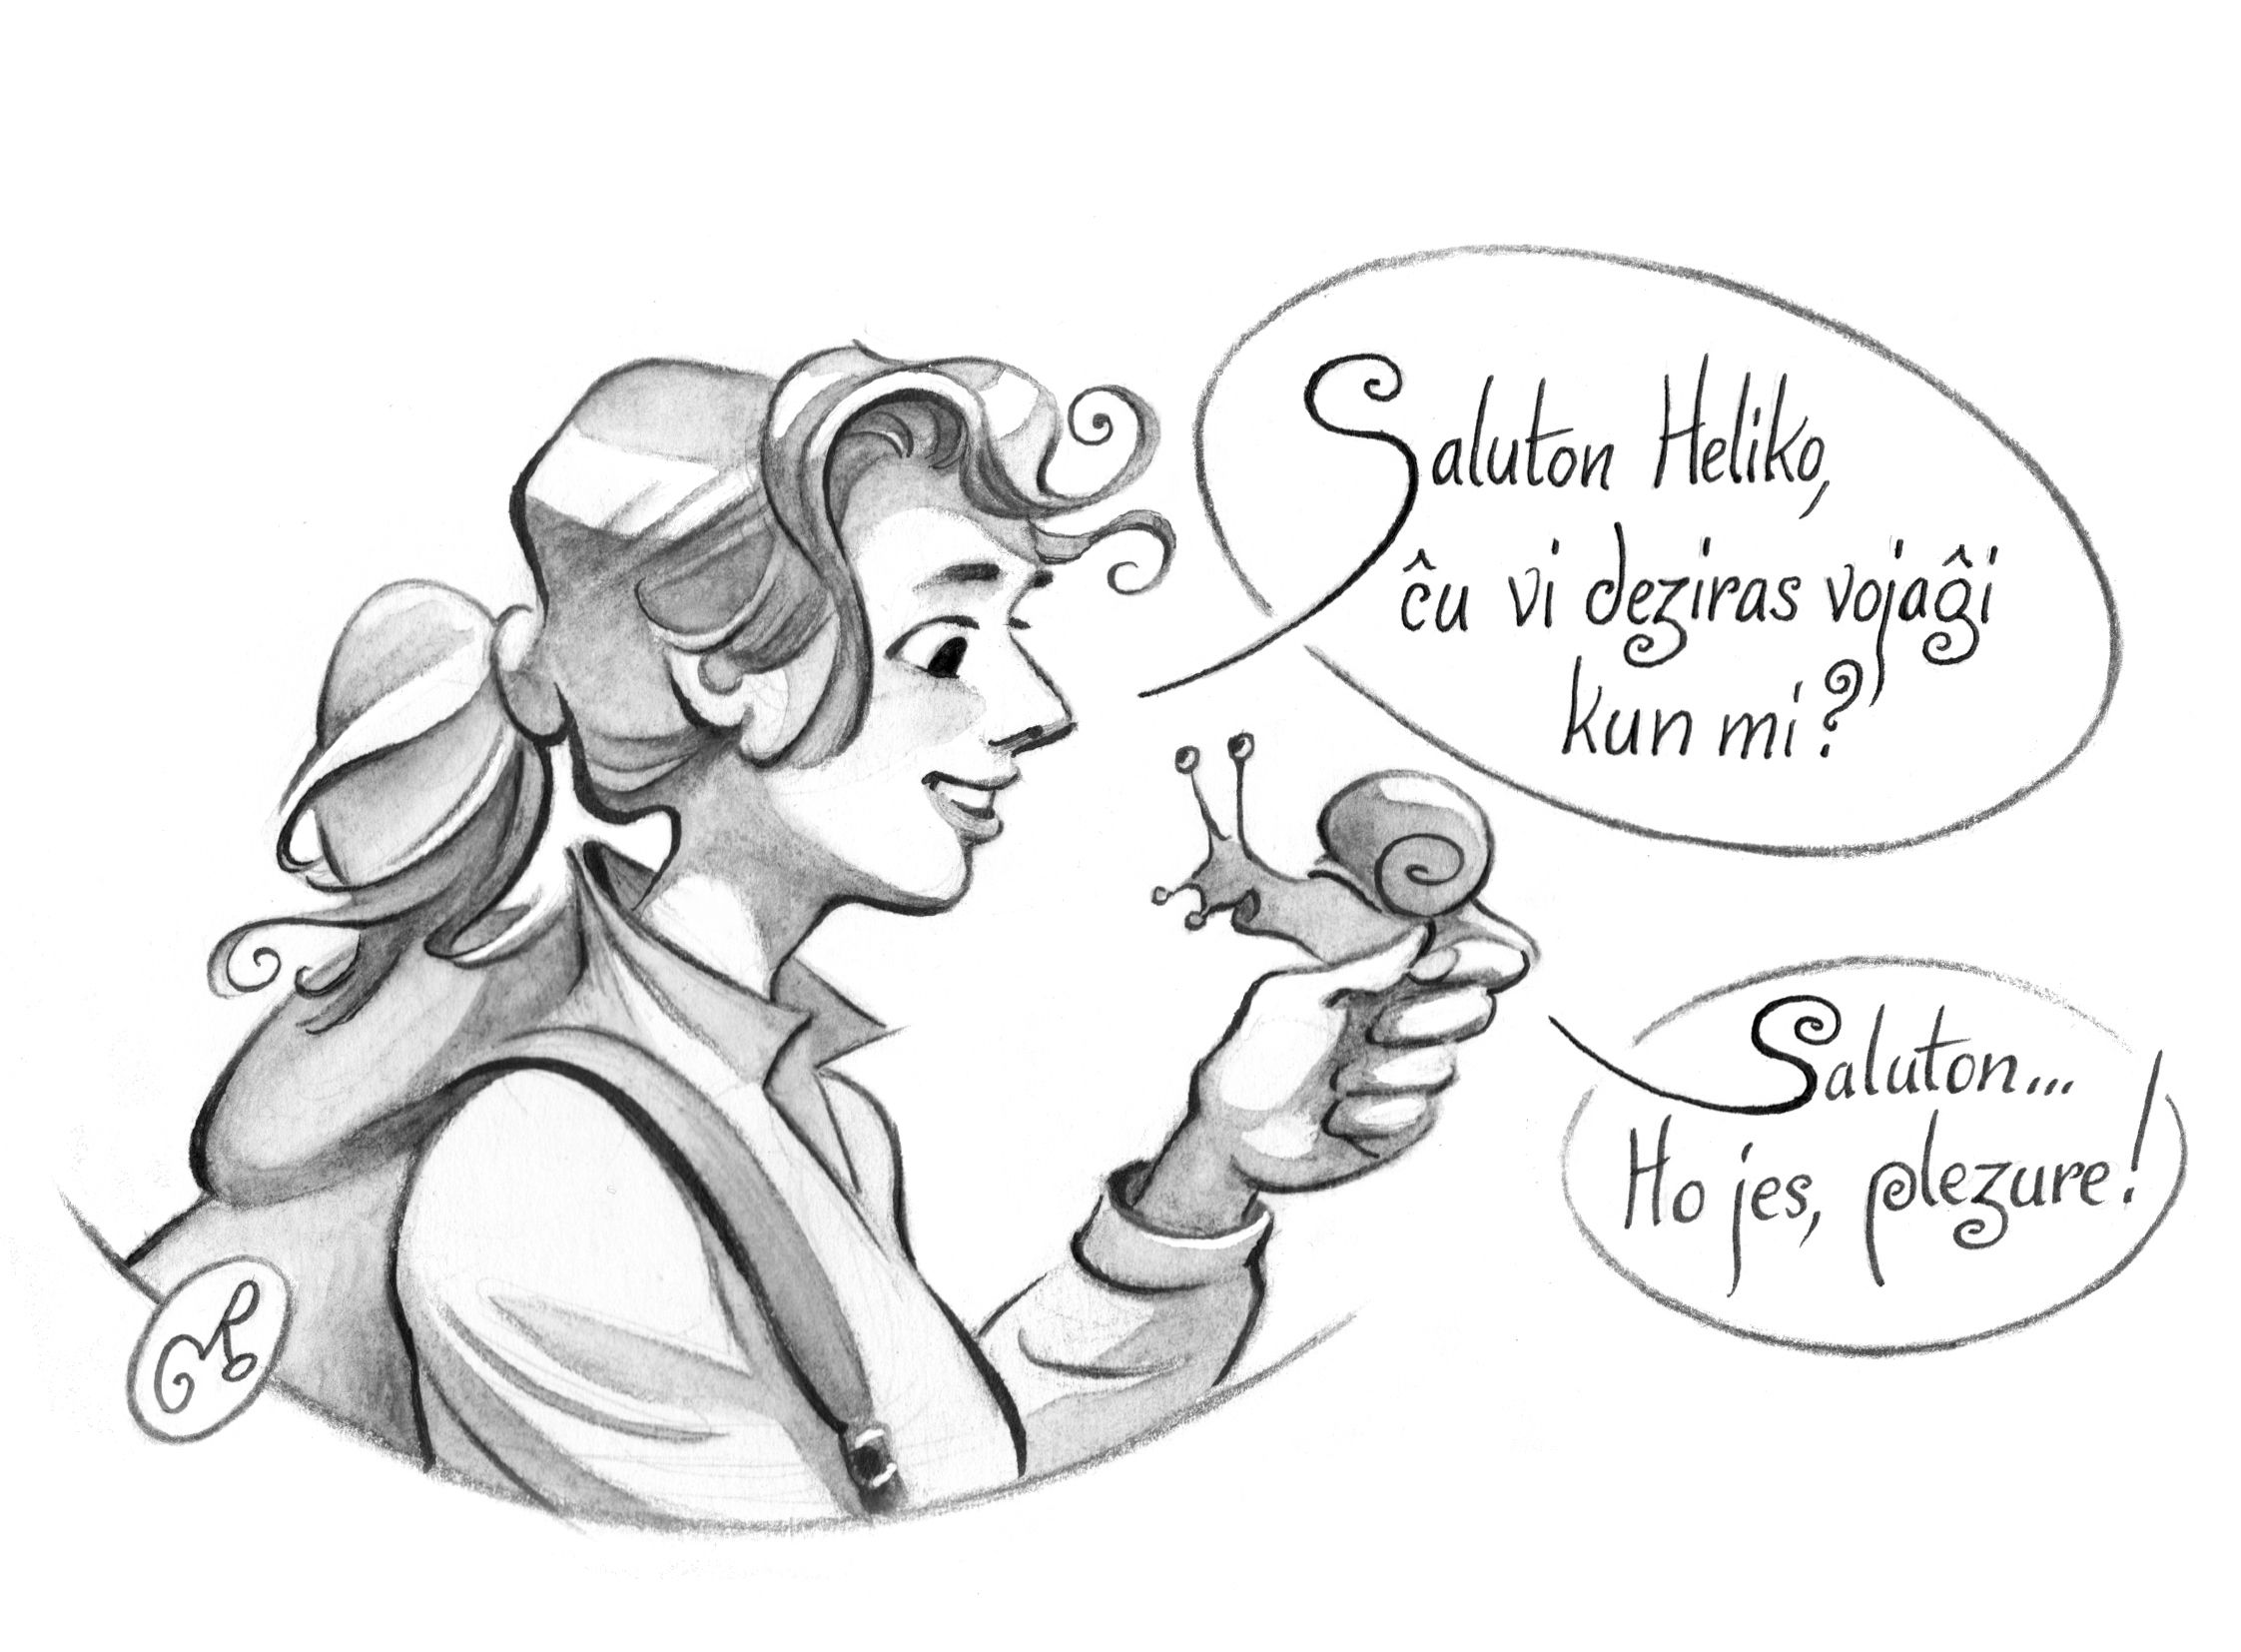
\includegraphics[width=\textwidth]{img/PS_2017_4_babilado.jpg}
\end{figure}

  
\end{document}
